%!TEX root=./LIVRO.tex
\chapter{Argumentar e convencer}
\markboth{Módulo 1}{}

\section{Habilidades do SAEB}

\begin{itemize}

  \item Identificar o uso de recursos persuasivos em textos verbais e não verbais.

  \item Identificar teses, opiniões, posicionamentos explícitos e argumentos em textos.

\end{itemize}

\subsection{Habilidades da BNCC} 

\begin{itemize}

  \item EF67LP05, EF67LP07.

\end{itemize}

\conteudo{Você já deve ter percebido que, o tempo todo, estamos expostos a
textos que pretendem nos convencer de alguma coisa --- da qualidade de um
produto, da verdade de uma informação ou da necessidade de uma conduta.

Para que seja convincente, o texto deve ter algumas características
específicas. Em primeiro lugar, a linguagem deve ser adequada ao público a que
se destina a informação. Não vale, por exemplo, escrever difícil, com
linguagem muito técnica ou vocabulário desconhecido, para crianças ou adultos
que não tiveram a chance de estudar. E o contrário também é verdadeiro: um
texto muito simples não é eficiente para convencer um professor universitário,
que é especializado em assuntos complexos.

Outra forma de convencer o leitor é usar recursos não verbais: as imagens
podem ajudar muito a ilustrar o que as palavras querem dizer. Existe até um
ditado que diz que ``uma imagem vale mais do que mil palavras''. E é verdade
mesmo: uma foto ou um gráfico podem ajudar muito a explicar e simplificar o
sentido de longas frases e parágrafos.

Detalhes como esses são importantes tanto na hora de escrever quanto na hora
de ler um texto argumentativo. É por meio de textos assim, repletos de dados e
estatísticas --- e principalmente de relações lógicas estabelecidas entre
essas informações --- que podemos formar nossas próprias opiniões e planejar
nossas ações no mundo.

Cada vez mais recebemos uma quantidade enorme de informações, de forma
imediata, por meio de aplicativos, da imprensa, de diferentes canais de
notícias e das redes sociais. Precisamos estar atentos a tais recursos e à
forma como somos influenciados por eles. É fundamental saber que \textbf{toda
comunicação parte de uma intenção}, mesmo que isso não apareça explicitamente
no texto. Com atenção, podemos reconhecer os recursos persuasivos em campanhas
publicitárias, debates políticos, discursos de vendas, em diversos tipos de
texto.}

%Paulo: este autor fez, ao final do conteúdo, extensas orientações ao professor. Coloquei-as todas em \coment{}
% \coment{Professor(a), relembre os principais gêneros textuais que utilizam
% recursos verbais e não verbais, questione gêneros conhecidos pelos alunos.
% Estimule os estudantes a pensar sobre os argumentos, mostre como podem servir
% para a formação de opinião no caso de textos jornalísticos, ou para
% convencimento, nos casos de textos publicitários. Relembre também a
% necessidade do rigor técnico no caso de textos de divulgação científica.

% Utilize exemplos distintos para explicar as funções dos recursos verbais e não
% verbais e estimule os estudantes na identificação das associações que podem
% ser feitas entre as imagens e as palavras. Chame a atenção para a citação dos
% órgãos oficiais e ressalte que esse tipo de referência pode tornar um texto
% mais ou menos confiável por conta da possibilidade de confrontar e questionar
% os dados apontados. Relembre os estudantes sobre o uso de recursos persuasivos
% em demais gêneros textuais, apontando também para suas especificidades quanto
% ao público alvo, função comunicativa e meios de veiculação.}

\section{Atividades}

\num{1} De acordo com seus conhecimentos, escreva dois tipos de recursos persuasivos presentes em campanhas publicitárias:

\reduline{1. Linguagem objetiva, clara e direta; 2. recursos verbais e não verbais;
3. escolha de fontes adequadas; 4. imagens que chamem a atenção do público alvo, entre outras.\hfill}

\num{2} Sobre os textos de divulgação científica assinale (V) para as afirmações verdadeiras e (F) para as afirmações falsas:

\begin{table}[h!]
\begin{tabular}{|c|l|}
\hline
\textbf{\begin{tabular}[c]{@{}c@{}}Verdadeiro (V)\\ ou \\ Falso (F)?\end{tabular}} & \multicolumn{1}{c|}{\textbf{Afirmação}} \\ \hline
\rosa{F} & Apresentam linguagem de difícil compreensão \\ \hline
\rosa{F} & Utilizam apenas recursos não verbais \\ \hline
\rosa{V} & Pretendem convencer \\ \hline
\rosa{V} & Apresentam linguagem objetiva \\ \hline
\end{tabular}
\end{table}

%\coment{F, F, V, V} Deixei o gabarito aqui caso minha tabela não funcione. (Rogério, 25/5/23, 15h15)

% Textos de divulgação científica apresentam linguagem clara e objetiva
% para divulgar conhecimentos científicos de forma acessível para o
% público em geral e neles podem-se utilizar recursos não verbais tais como gráficos
% e tabelas para apresentar os resultados descritos.

Leia a sentença a seguir e responda as questões 3 e 4. 

\begin{myquote}

A dieta vegetariana é muito mais saudável. Abandonar o consumo de carne de animais 
reduz o risco de colesterol alto, previne contra o câncer, aumenta a energia e ajuda a
controlar o peso.

\end{myquote}

\num{3} Qual a afirmação principal do texto?

\reduline{A afirmação principal é a de que a dieta vegetariana é mais saudável.\hfill}

\num{4} Quais argumentos sustentam a afirmação principal?

\reduline{Os argumentos que baseiam a afirmação principal são as afirmações de que  
a dieta vegetariana reduz o risco de colesterol alto, previne contra o câncer, aumenta
a energia e ajuda a controlar o peso.\hfill}

Leia a notícia abaixo e responda às questões de 5 a 10.

\begin{myquote}

\textbf{No Brasil, mulher é vítima de violência a cada quatro horas}

Um estudo de dados de sete estados brasileiros revela que, no ano de
2022, uma mulher tornou-se vítima de violência a cada quatro horas. Trata-se de 
um total de 2.423 casos de violência, dos quais 495 resultaram em morte.

É no estado de Pernambuco que ocorre o maior número de transfeminicídios ---
posição que estava nas estatísticas do Ceará nos últimos dois anos. De acordo 
com as conclusões da pesquisadora da Rede em Pernambuco, Dália Celeste, essa 
situação está diretamente relacionada à negligência por parte do governo. Ela 
aponta que houve falta de ação pública, mesmo
após uma grande onda de ataques transfóbicos em 2021. Celeste
destaca que os corpos de pessoas trans e travestis são frequentemente
submetidos a um processo de desumanização, sendo vistos como corpos que não
deveriam existir, o que contribui para o aumento dos crimes de ódio.

Mas a situação não é menos preocupante em outros estados: A Bahia destaca-se 
pela maior taxa de crescimento de feminicídios em comparação com o último relatório, 
apresentando um aumento significativo de 58\%. Esse estado registra pelo 
menos um caso por dia e, lamentavelmente, lidera as ocorrências no Nordeste, 
com um total de 91 registros. O Rio de Janeiro, por sua vez, alcançou a deplorável marca de
ao menos um caso de violência contra a mulher a cada 17 horas, e dobrou 
o número de casos de violência sexual, de 39 para 75.

\fonte{Texto formulado para este material. Fonte de pesquisa: 
https://g1.globo.com/rj/rio-de-janeiro/noticia/2023/03/06/
estudo-em-sete-estados-aponta-que-uma-mulher-e-vitima-de-violencia-a-cada-quatro-horas.ghtml
Acesso: 25 set. 2023}

\end{myquote}

\num{5} Sintetize o conteúdo da notícia usando apenas uma palavra. 

\reduline{Com base no título e no texto, pode-se sintetizar o conteúdo da notícia com 
a palavra ``feminicídio'', isto é, o assassinato de mulheres envolvendo violência 
doméstica e familiar, menosprezo ou discriminação à condição de mulher da vítima.\hfill}

\num{6} Podemos considerar que o título e o primeiro parágrafo contêm uma apresentação 
geral do texto. Explique essa afirmação com suas próprias palavras.

\reduline{Com base no título e no primeiro parágrafo, podemos afirmar que o conjunto do texto 
apresentará dados referentes ao feminicídio em todo o Brasil. É o que ocorre na informação
sintética do título, especificada no primeiro parágrafo, mas ainda referente ao país como
um todo. É somente no segundo e terceiro parágrafos que dados específicos de outros estados
serão apresentados. \hfill}

% REVER
% \begin{table}[h!]
% \begin{tabular}{ll} 
% (I) Ceará\\ 
% (II) Pernambuco & (\rosa{II}) O segundo colocado em número de casos de feminicídio.\\ (\rosa{II}) Estado onde ocorre pelo menos um caso a cada dois dias.\\ (\rosa{II}) O primeiro colocado em número de casos de transfeminícidio.\\ (\rosa{I}) O primeiro colocado em número de casos de transfeminicídio nos anos anteriores.
% \end{tabular}
% \end{table}

%\coment{(II) O segundo colocado em número casos de feminicídio. 
%(II) Estado onde ocorre pelo menos um caso a cada dois dias.
%(II) O primeiro colocado em número de casos de transfeminícidio.
%(I) O primeiro colocado em número de casos de transfeminicídio nos anos anteriores.}

\num{7} No segundo parágrafo, a notícia traz uma nova informação sobre violência contra mulher. 
Que informação é essa?

\reduline{A notícia traz novos dados sobre os casos de transfeminicídio --- isto é, 
os homicídios de mulheres trans. A pesquisa indica que o número dessas ocorrências em 
Pernambuco superou o do Ceará.\hfill}

\num{8} Segundo o texto da notícia, qual a principal motivação dos crimes de transfeminicídio
no estado de Pernambuco?

\reduline{Segundo a matéria, a negligência do governo em promover políticas públicas
contra os crimes de ódio é fator que influencia no aumento dos
casos no estado de Pernambuco.\hfill}

\num{9} O texto deixa claro que crimes de transfobia podem ser considerados um crime específico.
Que tipo de crime é esse? Segundo a pesquisadora citada no texto, o que incita esse tipo
de crime? 

\reduline{Segundo o texto, crimes de transfobia podem ser considerados crimes de ódio. Para
a pesquisadora Dália Celeste, a desumanização dos corpos trans e travestis contribui para que eles
sejam vistos como corpos que não deveriam existir, o que alimenta os crimes de ódio.\hfill} 

\num{10} Identifique, no segundo e terceiro parágrafos, recursos e expressões que permitem 
concluir qual é o ponto de vista do autor e explicite qual é a opinião dele sobre os feminicídios 
no Brasil   

\reduline{O autor do texto pretende denunciar o aumento do feminicído no Brasil. No segundo 
parágrafo, o autor dá voz a uma pesquisadora que se solidariza com as vítimas; no terceiro, frases e
expressões como ``a situação não é menos preocupante'', ``lamentavelmente'' e ``deplorável'' revelam
a oposição frontal do autor às ocorrências de feminicídio no Brasil.\hfill}

\section{Treino}

\num{1} Leia o texto abaixo para responder à questão.

\begin{myquote}

Nas Américas, a malária continua ameaçando a vida de cerca de 138 milhões de pessoas.
Para a erradicação dessa doença, é fundamental a cooperação entre os países atingidos e 
entre distintos setores da sociedade. É digno de nota que os males causados por essa doença
não se limitam apenas à saúde, mas também impactam a economia, as relações de trabalho e 
o meio-ambiente. Como os mosquitos transmissores da doença não respeitam fronteiras, a migração
de áreas endêmicas desempenha um papel significativo na propagação da malária. 

\end{myquote}

\fonte{Texto formulado para este material. Fonte de pesquisa:
https://www.paho.org/pt/noticias/4-11-2022-intervencoes-locais-sao-cruciais-para-atingir-objetivo-eliminacao-da-malaria.
Acesso em: 25 set. 2023.}

De acordo com o texto, a erradicação da malária se baseia na cooperação entre diferentes países 
da América porque:

\begin{escolha}

  \item a migração ajuda a espalhar a doença de um país para outro.

  \item os países da América não tem nenhuma meta para eliminar a doença.

  \item não há correlação entre casos de malária e migração. 

  \item o mundo da economia e do trabalho é pouco saudável.

\end{escolha}

\num{2} Leia o texto abaixo para responder à questão.

\begin{myquote}

Depois da queda de casos de \textsc{covid}-19, escolas públicas e privadas 
do Estado de São Paulo começaram a receber os estudantes. No entanto, em vez 
de dar prioridade ao acolhimento e à criação coletiva de novas abordagens para
organizar tempos, espaços, grupos e relações, muitas delas optaram por retornar 
à estrutura tradicional e enfatizaram as avaliações externas para ``diagnosticar 
as deficiências na aprendizagem''. O resultado dessa abordagem foi o aumento 
significativo de incidentes de violência e problemas de saúde tanto entre os
estudantes quanto os professores.

\end{myquote}

\fonte{Texto formulado para este material. Fonte de pesquisa: https://www.uol.com.br/ecoa/colunas/opiniao/2023/03/28/ataque-em-escola-policial-no-colegio-nao-e-solucao-para-evitar-tragedia.htm
Acesso em: 25 set. 2023.}

Para o autor do texto acima, quando receberam alunos e professores depois da pandemia de 
\textsc{covid}-19, as escolas deveriam: 

\begin{escolha}

  \item ensinar formas de organizar tempos, espaços, grupos e relações.

  \item priorizar a saúde de estudantes e professores por meio de palestras.

  \item amparar estudantes e professores e discutir com eles modos de organização.

  \item valorizar as tradições escolares, sobretudo as avaliações de deficiências.  

\end{escolha}

\num{3} Leia o texto abaixo para responder à questão.

\begin{myquote}

Uma alimentação saudável deve ser baseada em práticas alimentares que
assumam a significação social e cultural dos alimentos como fundamento
básico conceitual. Neste sentido é fundamental resgatar estas práticas
bem como estimular a produção e o consumo de alimentos saudáveis
regionais (como legumes, verduras e frutas), sempre levando em
consideração os aspectos comportamentais e afetivos relacionados às
práticas alimentares.

\end{myquote}

\fonte{Biblioteca Virtual em Saúde do Ministério da Saúde. Alimentação saudável. 
Disponível em: https://bvsms.saude.gov.br/alimentacao-saudavel/.
Acesso em: 19 mai. 2023.}

De acordo com as afirmações presentes no texto, é correto afirmar que a alimentação saudável
está diretamente relacionada

\begin{escolha}

  \item à cultura e às relações afetivas do consumidor.
  
  \item ao acesso a mercados e pontos de consumo.
  
  \item à difusão oficial de informações sobre alimentos.
  
  \item à produção e ao consumo de alimentos industriais.

\end{escolha}

\chapter{Os domínios da comunicação}
\markboth{Módulo 2}{}

\section{Habilidades do SAEB}

\begin{itemize}

  \item Identificar elementos constitutivos de textos pertencentes ao
domínio jornalístico/midiático.

  \item Identificar formas de organização de textos normativos, legais e/ou
reivindicatórios. Identificar elementos constitutivos de gêneros de
divulgação científica.

  \item Analisar a relação temática entre diferentes gêneros jornalísticos.

\end{itemize}

\subsection{Habilidades da BNCC}

\begin{itemize}
  
  \item EF69LP02, EF69LP20, EF69LP27, EF67LP16, EF67LP17.

\end{itemize}

\conteudo{Você já deve ter percebido que, no nosso dia a dia, temos de ler
diferentes tipos de texto, cada um deles com uma finalidade específica. Uma
reportagem em um site de notícias serve para a gente se informar. Uma receita
é um guia prático para fazer comidas saborosas. As placas de rua servem para
as pessoas se orientarem na cidade. E assim por diante.

Cada um desses textos pertence a diferentes \textbf{gêneros textuais}, que
devem ser adequados às muitas situações do cotidiano. Eles podem servir para
informar, formar opinião, persuadir, regulamentar, propor mudanças, fazer
reclamações, reivindicações ou solicitações. Em outras circunstâncias, servem
para registrar normas e leis, para garantir direitos a partir de mecanismos
legais e ainda podem ser usados para divulgação de pesquisas e resultados de
experimentos, por exemplo. O importante é saber que, para cada função
comunicativa, há um gênero adequado de texto.

Textos como editoriais, reportagens, notícias e crônicas fazem parte do
contexto jornalístico e têm características específicas: uma reportagem, por
exemplo, propõe-se a informar objetivamente --- em linguagem clara, destinada
ao maior número de pessoas --- o que aconteceu, com quem, quando, onde e por
quê. No universo legal ou jurídico, a linguagem dos textos deve ser técnica,
com vocabulário específico para garantia da clareza e precisão conceitual. Por
isso, textos normativos ou de âmbito legal são, em geral, bastante
padronizados. Eles pretendem propor ações jurídicas, argumentar e defender
pontos de vista e atitudes com base em disposições legais. Já os textos que
visam defender causas sociais, propor mudanças políticas e econômicas
--- tais como petições, manifestos e cartas abertas --- pertencem ao universo
da reivindicação e geralmente apresentam elementos persuasivos e de
convencimento sobre determinado ponto de vista. Por essa característica,
neste domínio encontramos também os discursos públicos e políticos.

Veja que curioso: textos científicos podem soar, muitas vezes,
incompreensíveis para o público em geral, devido ao rigor conceitual e ao
vocabulário muito específico. É interessante pensar que um pesquisador, ao
escrever um artigo científico, se dirige a um público especializado,
acostumado com aquela linguagem difícil para a maioria das pessoas. Mas esse
mesmo autor pode escrever um texto mais simples e publicá-lo no jornal,
destinado ao público em geral, com a finalidade de divulgar suas descobertas a
muito mais gente.

Concluindo: para cada situação de comunicação, existe um texto correspondente,
que é adequado ao contexto em que se insere e ao público a que se destina. O
bom autor e bom leitor são as pessoas que conseguem identificar os recursos
específicos do maior número de gêneros.}

% \coment{Professor, relembre com os estudantes as características dos gêneros
% citados:

% \textbf{Domínio jornalístico midiático}: Linguagem clara e direta. Este
% domínio tem peculiaridades como o uso de títulos, subtítulos, fotografias e
% vídeos. Para que um fato ou ocorrido seja bem noticiado, o autor deve oferecer
% aos leitores ou ouvintes os dados sobre o local, a data e um resumo direto do
% que está sendo comunicado. Textos deste domínio podem ainda conter ou não a
% opinião de quem escreve ou do veículo que disponibiliza o conteúdo.

% \textbf{Domínio legal ou jurídico}: Estes textos podem ser documentos,
% estatutos, códigos de legislação e servem para leis e demais documentos
% regulatórios. São divididos em parágrafos, seções e capítulos.

% \textbf{Textos de divulgação científica}: com a finalidade de promover a
% divulgação de pesquisas e resultados de trabalhos científicos baseados
% em estudos e práticas de observação.}

\section{Atividades}

Analise a imagem a seguir e responda às questões 1 e 2. 

\begin{longtable}[]{@{}l@{}}
\toprule
\endhead
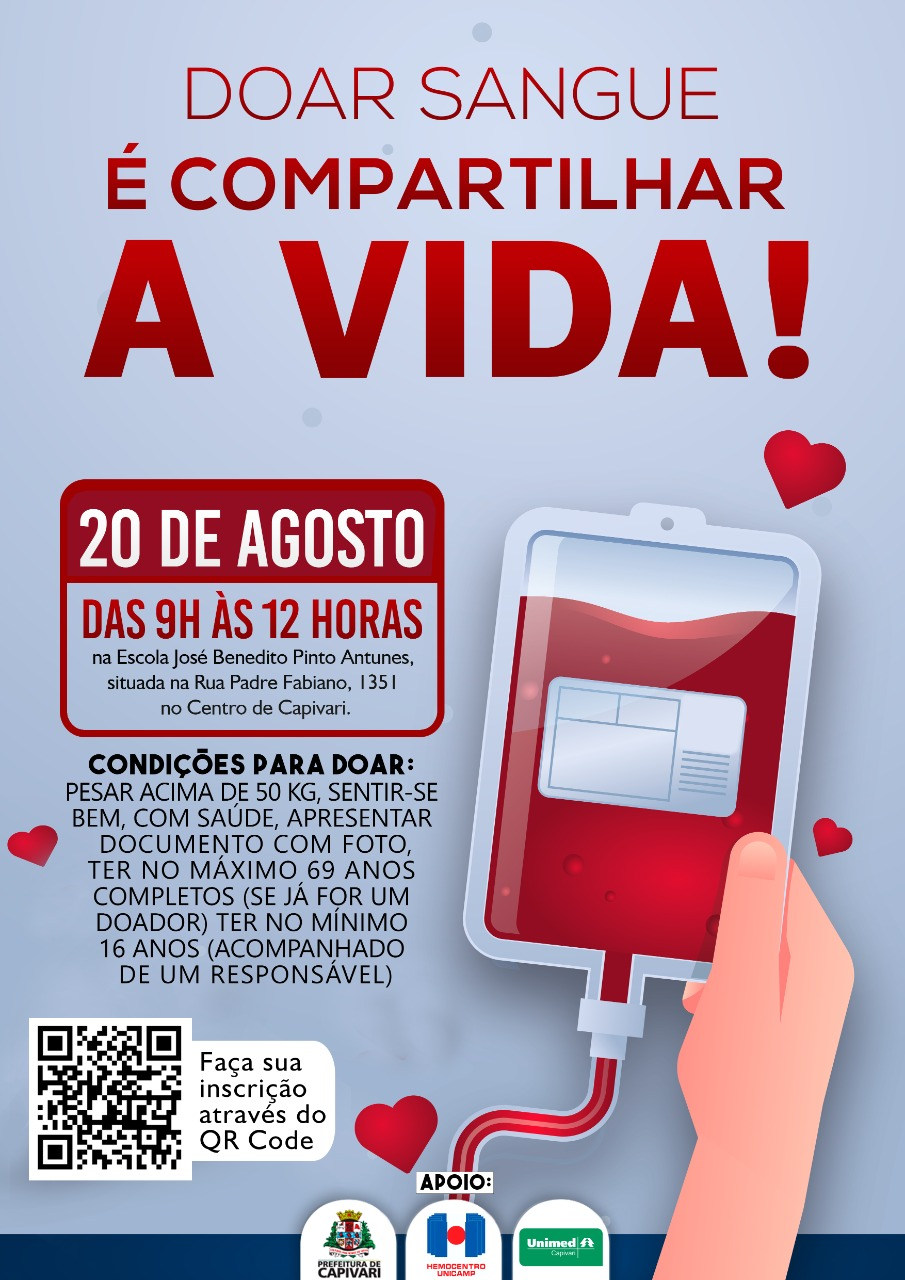
\includegraphics[width=5.76042in,height=8.15278in]{./imgSAEB_7_POR/media/image1.png} \\
\bottomrule
\end{longtable}

\fonte{Prefeitura de Capivari. Secretaria de Saúde anuncia Campanha de Doação de Sangue no dia 20 de agosto. Disponível em:
https://capivari.sp.gov.br/portal/secretaria-de-saude-anuncia-campanha-de-doacao-de-sangue-no-dia-20-de-agosto/
Acesso em: 19 mai. 2023.}

\num{1} A imagem contém uma campanha de conscientização. Sabendo que
o objetivo da campnaha é sensibilizar o público, aponte
recursos não verbais contribuem para a persuasão.

\reduline{Os recursos não verbais que contribuem para a persuasão são:
1. predomínio da cor vermelha no conjunto; 2. associação da imagem da bolsa de
sangue equiparada a um telefone para ilustrar o sentido da palavra
``compartilhar''; 3. caixa de destaque com informações de data e
horário.\hfill}

\num{2} Encontre no texto o verbo que indica uma recomendação de mudança 
de atitude. Escreva-o abaixo

\reduline{Os verbos ``doar'' e ``compartilhar'', no infitivo, sugerem mudança 
de atitude. O uso do verbo no infinitivo é uma característica do gênero. Para
incentivar uma atitude, o texto utiliza linguagem apelativa e multimodal.\hfill}

\num{3} Assinale com (V) verdadeiro ou (F) falso as afirmações a seguir sobre
\textbf{reportagens}, de gênero jornalístico e midiático:

\begin{table}[h!]
\begin{tabular}{|c|c|}
\hline
\textbf{\begin{tabular}[c]{@{}c@{}}Verdadeiro (V) \\ ou Falso (F)?\end{tabular}} & \textbf{Afirmação} \\ \hline
\rosa{V} & Apresentam linguagem direta \\ \hline
\rosa{F} & Contêm verbos no imperativo \\ \hline
\rosa{F} & Servem para divulgar conhecimentos \\ \hline
\rosa{V} & Têm como objetivo informar \\ \hline
\end{tabular}
\end{table}

%\coment{V, F, F, V}

Leia o seguinte trecho do Estatuto da Criança e do Adolescente -- ECA -- para 
responder às questões 4 e 5.

\begin{myquote}

\textsc{o presidente da república}: faço saber que o Congresso Nacional decreta e
eu sanciono a seguinte Lei: (\ldots{})

Título II: Dos Direitos Fundamentais (\ldots{})

Capítulo II: Do Direito à Liberdade, ao Respeito e à Dignidade (\ldots{})

Art. 16. O direito à liberdade compreende os seguintes aspectos:

I --- ir, vir e estar nos logradouros públicos e espaços comunitários,
ressalvadas as restrições legais;

II --- opinião e expressão;

III --- crença e culto religioso;

IV --- brincar, praticar esportes e divertir-se;

V --- participar da vida familiar e comunitária, sem discriminação;

VI --- participar da vida política, na forma da lei;

VII --- buscar refúgio, auxílio e orientação. \\

\end{myquote}

\fonte{Ministério dos Direitos Humanos e da Cidadania. O Estatuto da Criança e 
do Adolescente -- ECA.
Disponível em: http://www.gov.br/mdh/pt-br/navegue-por-temas/crianca-e-adolescente/publicacoes/o-estatuto-da-crianca-e-do-adolescente. Acesso em: 19 mai. 2023.}

\num{4} Identifique as características que indicam que o texto pertence à 
esfera jurídica.

\reduline{As características que indicam que o texto pertence à esfera jurídica 
são as seguinte: divisão em artigos e capítulos, uso de numerais romanos, uso de
linguagem formal, verbos no infinitivo.\hfill}

% \num{5} O uso do verbo no infinitivo em textos jurídicos e legais tem uma função. 
% Que função é essa?

% \reduline{Os verbos no infinitivo, no caso de textos de regulamentação, indicam
% orientação, têm uma função de persuadir, convencer ou convidar a uma
% ação ou atitude.\hfill}

Analise o texto a seguir para responder às questões 5 e 6. 

% Suprimi essa imagem porque ela não tem grande contribuição para o material. Rogério, 19/5/23, 16h21
%\begin{longtable}[]{@{}
%>{\raggedright\arraybackslash}p{(\columnwidth - 0\tabcolsep) * \real{0.9861}}@{}}
%\toprule
%\endhead
%\textbf{Alerta importante para você que é jovem e vai ler esta cartilha}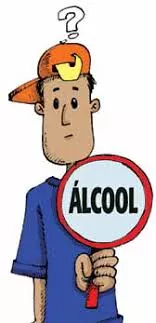
\includegraphics[width=1.625in,height=3.36458in]{./imgSAEB_7_POR/media/image2.png}

\begin{myquote}

O Estatuto da Criança e do Adolescente -- \textsc{eca} -- proíbe a venda de
qualquer tipo de bebida alcoólica para menores de 18 anos.

Portanto, fique esperto!

Se alguém lhe oferecer, mesmo que gratuitamente, qualquer bebida
alcoólica, \textsc{não aceite}!

Essa pessoa estará cometendo um crime.

É bom lembrar que o uso do álcool pode levar ao alcoolismo, uma doença
grave que atinge 12,3\% da população brasileira com idade entre 12 e 65
anos.

Entre os jovens de 12 a 17 anos, a taxa de alcoolismo é de 7\%.

Considere que este nível representa 554.000 jovens com sérios problemas
sociais e de saúde.

\end{myquote}

\fonte{Portal do Professor do Ministério da Educação. Drogas: Cartilha Álcool e Jovens. 
Disponível em: http://portaldoprofessor.mec.gov.br/storage/materiais/0000011863.pdf.
Acesso em: 2 de abri de 2023.}

\num{5} A quem se destina este texto? Explique e copie do texto um trecho que 
justifique sua resposta.

\reduline{O texto se destina a jovens, como se pode verificar por meio do
trecho ``Alerta importante para \textbf{você que é jovem} e vai ler esta
cartilha''.\hfill}

\num{6} Releia a frase: ``Considere que este nível representa 554.000 jovens
com sérios problemas sociais e de saúde.'' Que efeito persuasivo o autor 
alcançou ao utilizar o número absoluto que representa 7\% da população jovem?

\reduline{Ao apresentar o número absoluto de jovens que sofrem com 
problemas de alcoolismo, o autor se dirige direta e explicitamente 
ao público-alvo do texto, com o propósito de sensibilizá-lo.\hfill}

\num{7} No que diz respeito à linguagem, cite duas características comuns aos
gêneros jornalístico e de divulgação científica.

\reduline{Tanto no texto jornalístico quanto no de divulgação científica a
linguagem empregada deve ser clara e objetiva e pode haver o uso de
recursos não verbais tais como imagens, gráficos e tabelas.\hfill} 

Leia o texto abaixo e responda às questões 8 e 9. 

\begin{myquote}

\emph{Brasília, 23 de março de 2020}

Excelentíssimos(as) senhores(as), Presidente da República, Ministros de
Estado, Governadores(as), Prefeitos(as), Secretários(as) de Saúde e
gestores(as) do SUS,

O CNS, enquanto órgão responsável pelo controle social no SUS, orienta
que todos(as) os(as) referidos(as) nesta carta adotem medidas
emergenciais, em todas as unidades da federação, para os próximos dois
meses (abril e maio), visando conter a crise de saúde que vivemos hoje e
que pode se agravar nos próximos dias. O objetivo é zelar pela
integridade física e mental dos cidadãos e cidadãs brasileiros, buscando
também ações específicas e sensíveis à realidade de pessoas em regime
carcerário ou cumprindo medidas socioeducativas, dentre outras
populações vulneráveis. (\ldots{})

\emph{Conselho Nacional de Saúde} 

\end{myquote} 

\fonte{Conselho Nacional de Saúde. Carta aberta do CNS às autoridades 
brasileiras no enfrentamento ao Novo Coronavírus. Disponível em: https://conselho.saude.gov.br/ultimas-noticias-cns/1074-carta-aberta-do-cns-as-autoridades-brasileiras-no-enfrentamento-ao-novo-coronavirus.
Acesso em: 19 mai. 2023.}

\num{8} A quem se destina a carta?

\reduline{A carta se destina ao Presidente da República e aos Ministros 
de Estado, Governadores (as), Prefeitos(as), Secretários(as) de Saúde e gestores(as) do SUS.\hfill}

\num{9} Selecione do texto um trecho que expressa o motivo de reivindicação da carta.

\reduline{O trecho que expressa o motivo de reivindicação da carta é ``visando
conter a crise de saúde que vivemos hoje e que pode se agravar nos próximos
dias. Nesse sentido, é fundamental que sejam potencializadas ou desenvolvidas
as seguintes ações''.\hfill}

\num{10} Relacione os textos e suas características.

\begin{table}[h!]
\begin{tabular}{c|c|c|c|}
\cline{2-2} \cline{4-4}
 & \textbf{Texto} &  & \textbf{Característica} \\ \hline
\multicolumn{1}{|c|}{\textbf{1}} & \textbf{petição} & \rosa{1} & É um texto argumentativo de reivindicação \\ \hline
\multicolumn{1}{|c|}{\textbf{2}} & \textbf{estatuto} & \rosa{4} & Tem como objetivo divulgar informações \\ \hline
\multicolumn{1}{|c|}{\textbf{3}} & \textbf{folheto} & \rosa{3} & \begin{tabular}[c]{@{}c@{}}Utiliza recursos não verbais como \\ forma de persuasão\end{tabular} \\ \hline
\multicolumn{1}{|c|}{\textbf{4}} & \textbf{notícia} & \rosa{2} & Tem por objetivo regulamentar e normatizar \\ \hline
\end{tabular}
\end{table}

%Gabarito(1) É um texto argumentativo de reivindicação. (4) Tem como objetivo divulgar informações. (3) utiliza recursos não verbais como forma de persuasão. (2) tem por objetivo regulamentar e normatizar

\pagebreak

\section{Treino}

\num{1} Leia o texto abaixo para responder à questão.

\begin{myquote}

De acordo com o professor José Carlos Farah, as quedas em idosos são comuns
porque o processo de envelhecimento traz algumas perdas importantes no nosso
corpo.

``A osteopenia, que é a perda de massa óssea, deixa o osso enfraquecido, e a
perda da massa muscular, como consequência, traz a falta do controle do
movimento e equilíbrio, a perda cognitiva, que diminui a nossa atenção e
percepção e a baixa aptidão física''. Quando se soma isso a um quadro de
doenças preexistentes, o resultado é o de um cenário propício às quedas. Ainda
segundo o colunista, o processo de perdas do envelhecimento é inevitável. Mas
alguns hábitos podem ajudar e ele cita entre estes a prática da atividade
física. ``Os benefícios da prática da atividade física se contrapõem ao
processo de envelhecimento. O exercício promove o aumento da massa muscular e
da coordenação motora, do equilíbrio e das funções cognitivas. Este hábito já
diminui a possibilidade de quedas, associado ao ambiente livre de possíveis
obstáculos que podem atrapalhar o dia a dia do idoso''.

\end{myquote}

\fonte{José Carlos Simon Farah. Jornal da USP. Exercícios físicos podem contribuir 
para a redução da queda de idosos. Disponível em: https://jornal.usp.br/radio-usp/exercicios-fisicos-podem-contribuir-para-a-reducao-da-queda-de-idosos/.
Acesso em: 25 set. 2023. com adaptações.}

Pode-se afirmar que o trecho acima pertence a um texto de divulgação científica, pois contém:

\begin{escolha}
  
  \item informações técnicas voltadas ao público especializado da área médica.
  
  \item explicações de especialista sobre os benefícios do exercício físico para idosos.
  
  \item citações literais de artigos científicos sobre benefícios do exercício físico.
  
  \item narrativas pessoais sobre osteopenia em idosos e benefícios do exercício físico..

\end{escolha}

\num{2} Leia os dois textos a seguir para responder à questão. 

\begin{myquote}

%\textbf{Texto 1: ES registra aumento de casos de dengue na 1ª semana de janeiro}
% Em todo o mês de janeiro de 2022, o Espírito Santo teve 951
% casos. Só nesta primeira semana já foram 1.453. Infectologista acredita
% que estado pode estar vivendo uma epidemia de casos da doença.

% Só na primeira semana do ano foram registrados 1.453 casos da dengue no
% Espírito Santo. Número bem maior do que os registros do mês de janeiro
% de 2022, quando no mês todo foram registrados 951 casos da doença.

% Segundo o infectologista Crispim Cerutti, o estado pode estar vivendo
% uma epidemia da doença.

% ``A gente tem epidemias que ocorrem a aproximadamente a cada três anos. A
% última que a gente teve foi em 2019/2020. Embora o intervalo seja um
% pouco curto, a gente pode dizer que sim, estamos em uma nova epidemia da
% doença. A frequência de casos acompanha o ciclo de vida dos mosquitos'',
% explicou o infectologista.

\textbf{Texto 1}

No mês de janeiro de 2022, o estado do Espírito Santo registrou um
total de 951 casos de dengue. Surpreendentemente, apenas na primeira semana do
ano seguinte, já foram identificados 1.453 casos da doença. Esse aumento
significativo nas infecções levanta preocupações entre os especialistas em
doenças infecciosas, sugerindo a possibilidade de o estado estar enfrentando
uma epidemia da dengue.

Apenas nos primeiros sete dias do ano, o Espírito Santo já superou em muito o
número de casos relatados durante todo o mês de janeiro do ano anterior, que
totalizou 951 infecções. O doutor Crispim Cerutti, especialista em
infectologia, expressou sua preocupação com a situação e sugeriu que o estado
possa estar enfrentando uma epidemia.

O infectologista explicou que historicamente vivemos epidemias a
cada três anos, aproximadamente. A última aconteceu em 2019/2020.
Apesar de esse intervalo ser relativamente curto, Cerutti explica que 
é possível concluir que estamos enfrentando uma nova epidemia da doença. 
A frequência dos casos acompanha o ciclo de vida dos mosquitos transmissores.

\end{myquote}

\fonte{Texto formulado para este material. Fonte de pesquisa: https://g1.globo.com/es/espirito-santo/noticia/2023/01/18/es-registra-aumento-de-casos-de-dengue-na-1a-semana-de-janeiro.ghtml. Acesso em:
25 set. 2023.}

\textbf{Texto 2}

\begin{myquote}

Para evitar a reprodução do Aedes aegypti, o Ministério da Saúde recomenda 

\begin{itemize}
  
  \item Utilizar telas de proteção nas janelas de casa;
  
  \item Fechar portas e janelas;
  
  \item Manter o terreno limpo e livre de materiais ou entulhos;
  
  \item Tampar os tonéis e caixas d'água;
  
  \item Limpar as calhas regularmente;
  
  \item Tampar garrafas ou deixá-las com a boca para baixo;
  
  \item Manter lixeiras tampadas;
  
  \item Manter ralos limpos e com tela;
  
  \item Completar pratos de vasos de plantas com areia;
  
  \item Limpar com escova ou bucha os potes de água para animais;
  
  \item Limpar acessórios de decoração que ficam fora de casa 

  \item Evitar acúmulo de água em pneus e calhas;
  
  \item Usar repelentes elétricos ou naturais próximos às janelas;
  
  \item Evitar produtos de higiene com perfume, pois podem atrair insetos;
  
  \item Retirar água acumulada.
 
\end{itemize}

\fonte{Helio Carvalho. G1. Sete cidades da região de Campinas vivem situação de alerta para dengue; entenda o que significa.
Disponível em: https://g1.globo.com/sp/campinas-regiao/noticia/2023/01/17/sete-cidades-da-regiao-de-campinas-vivem-situacao-de-alerta-para-dengue-entenda-o-que-significa.ghtml. 
Acesso em: 19 mai. 2023.}

\end{myquote}

Os dois textos tratam de questões relacionadas à dengue. Quanto às diferenças
e semelhanças entre eles, assinale a alternativa correta:

\begin{escolha}

    \item Os dois exemplos pretendem informar a população sobre como evitar os casos de dengue.

    \item O primeiro apresenta uma notícia, e o segundo traz indicações de ações de prevenção.

    \item O primeiro exemplo é um texto de opinião; o segundo, um folheto informativo.

    \item O primeiro texto traz dados científicos sobre a dengue, e o segundo é um texto argumentativo.

\end{escolha}

\num{3} Leia os trechos extraídos da Constituição Brasileira de 1988 e responda
ao que se pede:

\begin{myquote}

\textbf{Trecho 1}

Art. 1.º A República Federativa do Brasil, formada pela união
indissolúvel dos Estados e Municípios e do Distrito Federal,
constitui-se em Estado democrático de direito e tem como fundamentos: (\ldots{})

Art. 3.º Constituem objetivos fundamentais da República Federativa do
Brasil:

IV - promover o bem de todos, sem preconceitos de origem, raça, sexo,
cor, idade e quaisquer outras formas de discriminação.

Art. 4.º A República Federativa do Brasil rege-se nas suas relações
internacionais pelos seguintes princípios:

III - autodeterminação dos povos;

\end{myquote}

\begin{myquote}

\textbf{Trecho 2}

Art. 215. O Estado garantirá a todos o pleno exercício dos direitos
culturais e acesso às fontes da cultura nacional, e apoiará e
incentivará a valorização e a difusão das manifestações culturais.

§ 1.º O Estado protegerá as manifestações das culturas populares,
indígenas e afrobrasileiras, e das de outros grupos participantes do
processo civilizatório nacional. 

Art. 216. Constituem patrimônio
cultural brasileiro os bens de natureza material e imaterial, tomados
individualmente ou em conjunto, portadores de referência à identidade, à
ação, à memória dos diferentes grupos formadores da sociedade
brasileira, nos quais se incluem:

I - as formas de expressão;

II - os modos de criar, fazer e viver;

III - as criações científicas, artísticas e tecnológicas;

IV - as obras, objetos, documentos, edificações e demais espaços
destinados às manifestações artístico-culturais;

V - os conjuntos urbanos e sítios de valor histórico, paisagístico,
artístico, arqueológico, paleontológico, ecológico e científico.

§ 1.º O poder público, com a colaboração da comunidade, promoverá e
protegerá o patrimônio cultural brasileiro, por meio de inventários,
registros, vigilância, tombamento e desapropriação, e de outras formas
de acautelamento e preservação. \\

\fonte{Constituição da República Federativa do Brasil.}
\end{myquote}

Sobre os trechos selecionados é correto afirmar que:

\begin{escolha}

  \item os dois trechos são contraditórios entre si.

  \item não há relação direta entre os dois trechos.

  \item os dois trechos versam sobre questões distintas.

  \item os dois trechos são complementares. 

\end{escolha}

\chapter{Nas tramas do texto literário}
\markboth{Módulo 3}{}

\section{Habilidades do SAEB}

\begin{itemize}
  
  \item Analisar elementos constitutivos de textos pertencentes ao domínio literário.
  
  \item Analisar a intertextualidade entre textos literários ou entre estes e outros textos 
verbais ou não verbais.
  
  \item Inferir a presença de valores sociais, culturais e humanos em textos literários.

\end{itemize}

\subsection{Habilidades da BNCC}

\begin{itemize}

  \item EF69LP44, EF69LP47, EF67LP27

\end{itemize}

\conteudo{Você já deve ter notado que a delícia de ler um texto 
literário é a possibilidade de encontrar mundos, pessoas e costumes
que a gente não conhece. Esse é uma das mais poderosas ferramentas
da ficção: por meio dela, em combinação com a nossa 
imaginação, a gente pode ir muito longe, a lugares possíveis
e até impossíveis, dependendo do caso. 

Uma das características mais fascinantes da literatura é que, ao 
mesmo tempo, ela é expressão de crenças, valores e ideias de determinada
sociedade. Da mesma maneira que nos leva longe, ela também
nos mostra características do que está perto de nós, de nossa
cultura. Por meio de textos literários, podemos observar hábitos, 
acontecimentos, desafios e questões de determinada época. A análise 
da literatura parte do texto, mas que encontra nele sentidos filosóficos,
sociológicos, históricos e antropológicos.

Ainda mais incrível é que alguns textos literários são tão ricos 
e tratam de temas tão essenciais e universais que acabam por sobreviver 
ao tempo. É fabuloso pensar que um texto escrito há mais de quinhentos
anos --- como as peças do inglês William Shakespeare, por exemplo ---
ainda pode ser interessante para um jovem leitor, como você. Não por 
acaso, marcas de \textbf{intertextualidade} permeiam a cultura
literária: trata-se de marcas indicadoras de que um autor está dialogando
com outros, do passado, seja para reafirmar o que fizeram, seja para 
superá-los. 

Por tudo isso, é fundamental o estudo de aspectos pertinentes à
linguagem, ao estilo, à estrutura e à temática das narrativas. 
A literatura tem o poder de despertar sensações,
questionamentos e proporcionar experiências estéticas que se refletem na
maneira como as pessoas escolhem ser e estar no mundo. O reconhecimento
do valor e da importância das obras do domínio literário pode
proporcionar uma formação ética e questionadora que participa da
formação cultural e intelectual da sociedade.}

% \coment{Professor(a), questione os estudantes sobre os gêneros textuais
% literários que conhecem, retome as principais características
% do conto, crônica, poesia, literatura de cordel, romance e demais
% gêneros que surgirem.

% Reforce a ideia de que tais gêneros retratam a sociedade com seus
% valores e desafios. Retome com os os estudantes os conhecimentos
% prévios sobre mitos, lendas e demais textos de origem popular e saliente
% a forma como os temas trabalhados remontam a hábitos, valores e crenças
% da cultura e da época em que foram escritos (lenda do milho, da
% mandioca, do arroz, sobre os rios, a paisagem, ritos de passagem,
% comemorações, etc). Chame a atenção dos estudantes para o
% fato de que os diversos tipos de artes podem se comunicar. Neste caso,
% pode ser citado como exemplo o texto dramático --- que
% pode ser lido, mas é escrito para ser encenado. Mostre como o teatro
% também promove integração de diversas expressões artísticas. Cite também
% outras expressões tais como a música e as artes plásticas e estimule os
% estudantes a pensarem como essas expressões se complementam.}

\section{Atividades}

\num{1} O conto popular é um gênero literário proveniente da tradição oral e
em sua textualidade mantém algumas marcas de estilo quanto à linguagem. Sobre
este aspecto da linguagem dos contos populares, cite duas marcas fundamentais
deste gênero.

\reduline{O gênero conto popular é marcado pela linguagem simples, direta e com
fortes traços de oralidade tais como regionalismos, gírias e expressões
populares.\hfill}

\num{2} Textos narrativos curtos e objetivos, baseados em eventos do
cotidiano: este gênero textual tem como objetivo divertir, entreter, provocar
reflexão ou fazer uma crítica. Qual gênero literário possui essas
características?

\reduline{As características apresentadas se referem à crônica, que traz questões 
cotidianas e pode conter traços de humor.\hfill}

Leia o trecho a seguir e responda as questões 3 e 4.

\begin{verse}

Disse Pedro isso é blasfêmia \\
É bastante astucioso \\
Pistoleiro e cangaceiro \\ 
Esse povo é impiedoso \\*
Não ganharão o perdão \\*
Do santo Pai Poderoso 

Inda mais tem sua má fama \\
Vez por outra comentada \\
Quando há um julgamento \\
Duma alma tão penada \\*
Porque fora violenta \\*
Em sua vida é baseada. 

\end{verse}

\fonte{Guaipuan Vieira. A chegada de lampião no céu. Disponível em: http://www.dominiopublico.gov.br/download/texto/rd000001.pdf.
Acesso em: 20 mai. 2023.}

\num{3} O texto acima pertence a qual gênero textual?

\reduline{O texto pertence à Literatura de Cordel.\hfill}

\num{4} Cite duas características do gênero presentes no trecho.

\reduline{Divisão em estrofes e versos, rima, métrica, temas da cultura
nordestina, no caso o personagem Lampião, marcas de oralidade.\hfill}

% \num{5} Use a legenda para indicar as características da crônica e do conto.
% Marque (1) para o crônica e (2) para o conto. Os dois podem ter
% características em comum:

% % Please add the following required packages to your document preamble:
% % \usepackage[table,xcdraw]{xcolor}
% % If you use beamer only pass "xcolor=table" option, i.e. \documentclass[xcolor=table]{beamer}
% \begin{table}[h]
% \begin{tabular}{cl}  %{| >{\columncolor[HTML]{DAE8FC}}c |l|}
% \hline
% \rosa{1, 2} & Poucos personagens \\ \hline
% \rosa{1, 2} & Curto e objetivo \\ \hline
% \rosa{1} & Histórias narram fatos do cotidiano e podem estimular a reflexão \\ \hline
% \rosa{2} & Podem surgir de narrativas populares transmitidos pela tradição oral \\ \hline
% \rosa{1} & É comum que seja publicado em jornais \\ \hline
% \end{tabular}
% \end{table}

Leia o trecho a seguir e responda às questões 5 e 6.

\begin{myquote}

Houve noutro tempo um rei que tinha o hábito de jogar, e todos com
quem jogava perdiam. Uma vez convidou a um outro rei para jogar, e, no
dia marcado, este se apresentou; mas perdeu todas as mãos do jogo, até
que se desenganou e despediu-se para se ir embora.

\end{myquote}

\fonte{Sílvio Romero. Contos Populares do Brasil. Coleção acervo brasileiro.
Volume 3, 2ª edição. Jundiaí: Cadernos do mundo inteiro, 2018 p. 128.}

\num{5} O que a expressão ``Houve noutro tempo'' quer dizer? Comumente outra
expressão é usada para iniciar os contos. Que expressão é essa?

\reduline{A expressão faz alusão a um tempo passado indeterminado. Nos contos é
comum que apareça a expressão ``Era uma vez'' com o mesmo significado de
tempo indeterminado.\hfill}

\num{6} Qual o tipo de narrador do trecho acima?

\reduline{O narrador do trecho é o narrador observador.\hfill}

\pagebreak
\num{7} Sobre a intertextualidade, assinale verdadeiro (V) ou falso (F) para as seguintes
afirmações.

\begin{table}[h!]
\begin{tabular}{|c|c|}
\hline
\textbf{\begin{tabular}[c]{@{}c@{}}Verdadeiro (V) \\ ou Falso (F)?\end{tabular}} & \textbf{Afirmação} \\ \hline
\rosa{F} & É a prática de copiar trechos de outras obras \\ \hline
\rosa{V} & \begin{tabular}[c]{@{}c@{}}É um recurso que pode trazer ainda mais \\ possibilidades de interpretação para um texto\end{tabular} \\ \hline
\rosa{V} & \begin{tabular}[c]{@{}c@{}}Pode estar implícita ou explícita em textos \\ e demais obras artísticas\end{tabular} \\ \hline
\rosa{V} & \begin{tabular}[c]{@{}c@{}}Pode estar presente em traduções, paródias \\ e releituras de obras\end{tabular} \\ \hline
\rosa{F} & Pode ser caracterizada como plágio \\ \hline
\end{tabular}
\end{table}

%\coment{F, V, V, V, F}

\num{8} No trecho abaixo vemos um exemplo de discurso indireto:

\begin{myquote}

O pai explicou: 
--- Filha, você precisa fazer sua tarefa agora. Mais tarde
temos compromisso.

\end{myquote}

Passe a frase para o discurso indireto.

\reduline{O pai explicou para a filha que ela precisava fazer a tarefa naquele
momento, pois, mais tarde, eles tinham compromisso.\hfill}

\section{Treino}

\num{1} Leia o texto abaixo para responder à questão.

\begin{myquote}

\textbf{Lenda da Mandioca}

\emph{Lenda Indígena}

Era uma vez uma índia chamada Atiolô. Quando o chão começou a ficar
coberto de frutinhas de murici, ela se casou com Zatiamarê. As frutinhas
desapareceram, as águas do rio subiram apodrecendo o chão. Depois, o sol
queimou a terra, um ventinho molhado começou a chegar do alto da serra.
Quando os muricis começaram outra vez a cair, numa chuvinha amarela,
Atiolô começou a rir sozinha. Estava esperando uma menininha.

\end{myquote}

\fonte{Ana Rosa Abreu e outros autores. Contos tradicionais, fábulas,
lendas e mitos. Disponível em http://www.dominiopublico.gov.br/download/texto/me001614.pdf. Acesso em: 20 mai. 2023)}

Nesse trecho da lenda da mandioca, notam-se traços da cultura
indígena com relação ao modo de explicar a origem dos alimentos, a
origem da natureza, a preservação dos costumes e a contagem do tempo.
Pode-se notar que a fruta murici é indicadora da passagem de certo 
período de tempo. Assinale a alternativa que explica corretamente 
quanto tempo se passou.

\begin{escolha}

  \item É possível concluir que cerca de um ano se passou.
  
  \item Não se pode saber ao certo quanto tempo se passou.
  
  \item A mudança de estação indica a passagem de três meses.  
  
  \item É legítimo pressupor que muitos anos se passaram. 

\end{escolha}

\num{2} Leia os poemas abaixo para responder à questão. 

\begin{myquote}

\textbf{Texto I: Canção do exílio}

\emph{Gonçalves Dias}

\begin{verse}

Minha terra tem palmeiras, \\

Onde canta o Sabiá; \\

As aves, que aqui gorjeiam, \\

Não gorjeiam como lá. 


Nosso céu tem mais estrelas,\\

Nossas várzeas têm mais flores, \\

Nossos bosques têm mais vida, \\

Nossa vida mais amores.


Em cismar, sozinho, à noite, \\

Mais prazer eu encontro lá; \\

Minha terra tem palmeiras, \\

Onde canta o Sabiá. \\


Minha terra tem primores, \\

Que tais não encontro eu cá; \\

Em cismar -- sozinho, à noite -- \\

Mais prazer eu encontro lá; \\

Minha terra tem palmeiras, \\

Onde canta o Sabiá. 


Não permita Deus que eu morra, \\

Sem que eu volte para lá; \\

Sem que desfrute os primores \\

Que não encontro por cá; \\

Sem qu'inda aviste as palmeiras, \\

Onde canta o Sabiá.

\end{verse}

\fonte{Gonçalves Dias. Primeiros Cantos. Disponível em:
http://www.dominiopublico.gov.br/download/texto/bn000100.pdf.
Acesso em: 6 abr de 2023.}

\end{myquote}

\begin{myquote}

\textbf{Texto II: Canção do exílio}

\emph{Murilo Mendes}

\begin{verse}

Minha terra tem macieiras da Califórnia \\

onde cantam gaturamos de Veneza. \\

Os poetas da minha terra \\

são pretos que vivem em torres de ametista, \\

os sargentos do exército são monistas, cubistas, \\

os filósofos são polacos vendendo a prestações. {[} \ldots{} {]} \\

Ai quem me dera chupar uma carambola de verdade \\

e ouvir um sabiá com certidão de idade!

\end{verse}

\end{myquote}

\fonte{Murilo Mendes. Poesias. Rio de Janeiro: José Olympio, 1959.}

A primeira versão da ``Canção do exílio'', escrita por Gonçalves Dias em 1847, tornou-se
importante obra do Romantismo brasileiro. Posteriormente, em 1930, o
poeta modernista Murilo Mendes retomou a poesia de Gonçalves Dias e
criticou as influências estrangeiras na cultura brasileira
apropriando-se do nacionalismo do Romantismo, transpondo-o para o
nacionalismo modernista. Sobre esta relação de
intertextualidade em obras literárias assinale a alternativa correta.

\begin{escolha}

  \item O poema de Murilo Mendes é um plágio do poema de Gonçalves Dias.

  \item O poema de Murilo Mendes não se refere ao poema de Gonçalves Dias.

  \item O poema de Murilo Mendes é uma paródia do poema de Gonçalves Dias.

  \item O poema de Gonçalves Dias é uma paródia do poema de Murilo Mendes.

\end{escolha}

\num{3} Leia o poema abaixo para responder à questão.


\includegraphics[width=4.11458in,height=2.80208in]{./imgSAEB_7_POR/media/image3.png}

\fonte{OBRANOME. Catálogo. Caixa Econômica Federal e
Embaixada da Espanha, no Conjunto Cultural da Caixa, Brasília, 2003.}

O texto acima pode ser caracterizado como poema visual. Os poemas visuais
foram amplamente explorados pelos poetas do concretismo e contêm
características próprias. Sobre as características da poesia concreta,
assinale a alternativa correta.

\begin{escolha}

  \item A combinação de palavras e imagens é irrelevante para a criação dos sentidos do poema. 

  \item Regras rígidas para a estrutura em versos rimados e estrofes caracterizam a poesia visual.

  \item Imagens ilustrativas não têm relação com os sentidos propostos pelo autor.

  \item A disposição de letras e palavras na página é recurso de produção de sentidos do poema.

\end{escolha}

\chapter{Formas de composição do sentido}
\markboth{Módulo 4}{}

\section{Habilidades do SAEB}

\begin{itemize}
  
  \item Analisar efeitos de sentido produzido pelo uso de formas de apropriação 
  textual (paráfrase, citação etc.).
  
  \item Analisar os efeitos de sentido decorrentes dos mecanismos de construção 
  de textos jornalísticos/midiáticos.

\end{itemize}


\subsection{Habilidades da BNCC}

\begin{itemize}

  \item EF69LP16, EF69LP43.

\end{itemize}

\conteudo{Há muitos elementos utilizados para argumentação em textos.
Por meio da estrutura do texto, da escolha de palavras e de recursos de estilo,
é possível perceber objetivos e intenções do autor. Os textos argumentativos
-- tais como artigos de opinião, editoriais ou discursos -- apresentam em sua
construção elementos que visam convencer de alguma ideia ou expor determinado 
ponto de vista. Para atingir esse objetivo, o autor se vale da coesão e da 
coerência. Com argumentos consistentes, bem concatenados e ideias claras, 
é possível encaminhar ao leitor as ideias almejadas. Existem recursos adequados
para persuadir ou convencer o
leitor: é o caso de argumentos de especialistas, dados de pesquisas ou exemplos,
entre muitos outros. Toda pessoa que deseja comunicar algo faz uso desses
recursos: no âmbito pessoal, em conversas informais entre colegas e familiares;
no âmbito profissional, em negociações e reuniões; no âmbito político, em
discursos; no âmbito estudantil e acadêmico, na elaboração de teses,
dissertações e apresentações de trabalho. Portanto, saber reconhecer e
utilizar recursos de persuasão e convencimento é fundamental para a 
convivência em sociedade e para a resolução de conflitos nos quais há a
necessidade discursos claros e orientados por argumentos. 

Para cada gênero textual, existem recursos comuns que auxiliam na boa
comunicação, de acordo com a finalidade e intenção do comunicador.
Dentre eles, o uso de aspas para introduzir citações, o uso de exemplos
para produzir argumentos, a escolha das palavras e de expressões de
acordo com o receptor.}

% \coment{Professor(a), relembre os estudantes sobre a necessidade de persuasão e
% convencimento nos gêneros textuais já estudados. É comum que relacionem
% a persuasão aos textos publicitários, mas vá além e discuta recursos de
% convencimento também em textos de opinião e em situações cotidianas.}

\section{Atividades}

Leia o texto abaixo para responder as questões:

\begin{myquote}

\textbf{Especialistas indicam formas de combate a atos de intimidação}

Um em cada dez estudantes brasileiros é vítima de bullying -- anglicismo
que se refere a atos de intimidação e violência física ou psicológica,
geralmente em ambiente escolar. O dado foi divulgado esta semana pelo
Programa Internacional de Avaliação de Estudantes (Pisa) 2015.

Especialistas, como a professora de psicologia Ciomara Shcneider,
psicanalista de crianças e adolescentes, defendem que pais e escola
devem estar atentos ao comportamento dos jovens e manter sempre abertos
os canais de comunicação com eles. Para ela, o diálogo continua a ser a
melhor arma contra esse tipo de violência, que pode causar efeitos
devastadores em crianças e adolescentes.

A Lei nº 13.185, em vigor desde 2016, classifica o bullying como
intimidação sistemática, quando há violência física ou psicológica em
atos de humilhação ou discriminação. A classificação também inclui
ataques físicos, insultos, ameaças, comentários e apelidos pejorativos,
entre outros.

``Os casos de bullying começam muito mais silenciosos e, por isso, são
mais graves. Quem sofre a agressão não conta nem na escola nem na
família, mas começa a mudar o comportamento'', explica. De acordo com
ela, queda no rendimento escolar, faltas na escola e mudanças no
comportamento são os sinais mais frequentes apresentados por quem sofre
esse tipo de violência. Por isso, família e escola devem estar sempre
atentos para os sinais que são apresentados pelos jovens.

Os mesmos cuidados, alerta a psicóloga, valem para situações enfrentadas
fora da escola, seja no mundo virtual -- como em casos de cyberbullying
--, na vizinhança onde moram ou nos locais que costumam frequentar.

\end{myquote}

\fonte{Ministério da Educação}

\num{1} Qual o principal assunto abordado no texto?

\reduline{O assunto do texto é o bullying.\hfill}

\num{2} Cite um elemento do texto que traz maior confiabilidade às informações.

\reduline{Discursos de autoridade, exemplos, dados de pesquisas e institutos de
pesquisa conferem credibilidade ao conjunto do texto e às informações nele 
contidas.\hfill}

\num{3} Qual a função do travessão no primeiro parágrafo do texto?

\reduline{A função do travessão é explicar o termo bullying.\hfill}

\num{4} Transcreva do texto o trecho em que a especialista oferece recursos
para lidar contra esse tipo de violência. 

comnet{O trecho solicitado é ``Para ela, o diálogo continua a ser a melhor
arma contra esse tipo de violência, que pode causar efeitos devastadores em
crianças e adolescentes.''}

\num{5} Utilize a legenda para classificar os tipos de argumento selecionados:

% Please add the following required packages to your document preamble:
% \usepackage[table,xcdraw]{xcolor}
% If you use beamer only pass "xcolor=table" option, i.e. \documentclass[xcolor=table]{beamer}
\begin{table}[h!]
\begin{tabular}{lp{7cm}} %{| >{\columncolor[HTML]{DAE8FC}}l |l|}
\hline
\textbf{(I) Argumento por Provas Concretas} & \begin{tabular}[c]{@{}p{7cm}}(\ )\small Especialistas, como a professora de psicologia Ciomara Shcneider,\\ psicanalista de crianças e adolescentes, defendem que pais e escola\\ devem estar atentos ao comportamento dos jovens e manter sempre abertos\\ os canais de comunicação com eles.\end{tabular} \\ \hline
\textbf{(II) Argumento de Autoridade} & \begin{tabular}[c]{@{}p{7cm}}(\ )\small Um em cada dez estudantes brasileiros é vítima de bullying -\\ anglicismo que se refere a atos de intimidação e violência física ou\\ psicológica, geralmente em ambiente escolar. O dado foi divulgado esta\\ semana pelo Programa Internacional de Avaliação de Estudantes (Pisa)\\ 2015.\end{tabular} \\ \hline
\textbf{(III) Argumento por Exemplificação} & \begin{tabular}[c]{@{}p{7cm}}(\ )\small A Lei nº 13.185, em vigor desde 2016, classifica o bullying como \\ intimidação sistemática, quando há violência física ou psicológica em\\ atos de humilhação ou discriminação. A classificação também inclui\\ ataques físicos, insultos, ameaças, comentários e apelidos pejorativos,\\ entre outros.\end{tabular} \\ \hline
\end{tabular}
\end{table}

\coment{% Please add the following required packages to your document preamble:
% \usepackage[table,xcdraw]{xcolor}
% If you use beamer only pass "xcolor=table" option, i.e. \documentclass[xcolor=table]{beamer}
% \begin{table}[h!]
% \begin{tabular}{|l|l|} %{| >{\columncolor[HTML]{DAE8FC}}l |l|}
% \hline
% \textbf{(I) Argumento por Provas Concretas} & \begin{tabular}[c]{@{}l@{}}(II) Especialistas, como a professora de psicologia Ciomara Shcneider,\\ psicanalista de crianças e adolescentes, defendem que pais e escola\\ devem estar atentos ao comportamento dos jovens e manter sempre abertos\\ os canais de comunicação com eles.\end{tabular} \\ \hline
% \textbf{(II) Argumento de Autoridade} & \begin{tabular}[c]{@{}l@{}}(I) Um em cada dez estudantes brasileiros é vítima de bullying -\\ anglicismo que se refere a atos de intimidação e violência física ou\\ psicológica, geralmente em ambiente escolar. O dado foi divulgado esta\\ semana pelo Programa Internacional de Avaliação de Estudantes (Pisa)\\ 2015.\end{tabular} \\ \hline
% \textbf{(III) Argumento por Exemplificação} & \begin{tabular}[c]{@{}l@{}}(III) A Lei nº 13.185, em vigor desde 2016, classifica o bullying como \\ intimidação sistemática, quando há violência física ou psicológica em\\ atos de humilhação ou discriminação. A classificação também inclui\\ ataques físicos, insultos, ameaças, comentários e apelidos pejorativos,\\ entre outros.\end{tabular} \\ \hline
% \end{tabular}
% \end{table}
}

\num{6} Copie do texto o trecho em que a especialista explica outro tipo de violência associada ao bullying que ocorre fora da escola

\reduline{O trecho solicitado é ``Os mesmos cuidados, alerta a psicóloga, valem
para situações enfrentadas fora da escola, seja no mundo virtual -- como em
casos de cyberbullying --, na vizinhança onde moram ou nos locais que costumam frequentar.\hfill}

\num{7} Qual o sinal usado para marcar as falas da especialista?

\reduline{O sinal usado para marcar as falas da especialista são as aspas.\hfill}

\num{8} No trecho ``De acordo com ela, queda no rendimento escolar, faltas na
escola e mudanças no comportamento são os sinais mais frequentes
apresentados por quem sofre esse tipo de violência.'' O pronome \textbf{ela} se
refere a quem?

\reduline{O pronome se refere à professora de psicologia Ciomara Shcneider.\hfill}

\num{9} A paráfrase é um recurso muito comum em textos de opinião e
argumentativos. Este recurso visa a reescrita de alguma fala ou
citação sem que seja necessária a referência direta. Retire do texto
um exemplo de paráfrase.

\reduline{O trecho a seguir contém paráfrase: ``Para ela, o diálogo continua a ser a
melhor arma contra esse tipo de violência, que pode causar efeitos devastadores
em crianças e adolescentes.''\hfill}

\num{10} Reescreva em forma de paráfrase a seguinte fala da especialista: ``Os 
casos de bullying começam muito mais silenciosos e, por isso, são mais graves. 
Quem sofre a agressão não conta nem na escola nem na família, mas começa a mudar 
o comportamento''

\reduline{A professora de psicologia explica que por ocorrerem de maneira
silenciosa, os casos de bullying podem ser mais graves. A vítima pode
apresentar mudanças de comportamento e pode não comunicar a escola e a
família sobre as agressões.\hfill}

\section{Treino}

\num{1} Leia o texto a seguir para responder à questão.

\begin{myquote}

\textbf{Como celulares mudaram nossos cérebros}

Como muitos de nós, passo tempo demais no meu celular. E, como muitos de
nós, sou totalmente consciente e costumo me sentir culpada por isso.

Às vezes, deixo o telefone no outro lado da casa ou o desligo, para usar
menos. Mas, no fim, acabo atravessando o corredor mais cedo do que
gostaria de admitir, para fazer algo que só posso fazer com o celular --
ou que ele me permite fazer com mais eficiência.

Há 50 anos, Martin ``Marty'' Cooper fez a primeira chamada de um
telefone móvel. Ele mesmo fabricou o aparelho -- um telefone bege, do
tamanho de um tijolo, muito diferente dos smartphones atuais, que são
finos e revestidos de vidro.

O aparelho de Cooper não tinha câmera e não enviava mensagens de texto.
Hoje, ele não pensa nos smartphones modernos como um aparelho
para fazer chamadas telefônicas.

``Realmente, ele não é um telefone muito bom em muitos aspectos'',
afirma Cooper. ``Pense um pouco. Você pega um pedaço de plástico e
vidro, que é plano, e coloca contra a curvatura da sua cabeça. Sua mão
fica em uma posição desconfortável.''

\end{myquote}

\fonte{A Gazeta.}

Sobre as vozes do texto, assinale a alternativa correta:

\begin{escolha}
  
  \item O texto apresenta a voz do autor e dos usuários de smartphone.
  
  \item O texto apresenta a voz dos criadores e usuários do smartphone.
  
  \item O texto apresenta as vozes do autor e do criador do primeiro telefone móvel.
  
  \item O texto apresenta a voz dos usuários de smartphones e do autor.

\end{escolha}

\num{2} Leia o texto abaixo para responder à questão.

\begin{myquote}

Os especialistas apontam a vida diante de uma tela como o principal dos
problemas. ``A revolução digital transformou os padrões de movimento das
pessoas e o modo como de se trabalhar, se divertir, aprender e viajar'',
sentencia num artigo, também na \textit{The Lancet}, Mark S. Tremblay,
especialista em vida saudável e obesidade do Instituto de Pesquisas do
Hospital de Ottawa (Canadá).

\end{myquote}

\fonte{Patrícia Peiró. El País Brasil. Sedentários e grudados a uma tela. Disponível em:
\url{https://brasil.elpais.com} Acesso em: 21 mai. 2023.}

O uso de aspas no texto acima é indicativo de:

\begin{escolha}

  \item introdução da fala do autor.

  \item destaque para a explicação.

  \item citação de um artigo.

  \item citação da fala de um especialista.

\end{escolha}


\num{3} Leia a manchete a seguir para responder à questão. 

Uso massivo de máscaras pode 'impedir segunda onda de covid-19', diz
estudo.

\fonte{BBC News Brasil. Uso massivo de máscaras pode 'impedir segunda onda de
covid-19', diz estudo. Disponível em: https://www.bbc.com/portuguese/geral-53058930.
Acesso em: 21 mai. 2023.}

Qual dos seguintes elementos da manchete contribui para sensibilizar o leitor 
quanto à necessidade prevenção contra a Covid-19? Assinale a alternativa correta.

\begin{escolha}

  \item O uso massivo de máscaras pela população.

  \item A possibilidade de impedir a segunda onda.

  \item A ameaça de haver uma segunda onda.

  \item A referência a um estudo científico.

\end{escolha}


\chapter{Informações implícitas no texto: fato ou opinião}
\markboth{Módulo 5}{}

\section{Habilidades do SAEB}

\begin{itemize} 

  \item Inferir informações implícitas em distintos textos.

  \item Distinguir fatos de opiniões em textos.

\end{itemize}

\subsection{Habilidades da BNCC}

\begin{itemize} 

  \item EF67LP04.

\end{itemize} 

\conteudo{Com a rápida expansão da tecnologia digital nas últimas décadas, a
quantidade de informação disponível e acessível está cada vez maior. Em
nenhum outro momento da história, houve tanto acesso a vídeos, imagens,
propagandas, opiniões, artigos acadêmicos, notícias e reportagens,
tutoriais, dentre tantos outros conteúdos. Há que se ter em mente, contudo,
que a crescente quantidade de informações não garante a qualidade dos
conteúdos gerados e distribuídos de maneira vertiginosa pela internet.
Mais do que nunca se faz necessário aprender a distinguir fatos de
opiniões, fontes confiáveis e fontes questionáveis, argumentos sólidos
de opiniões convincentes. Portanto, saber identificar em um texto as
marcas de subjetividade e objetividade, a intertextualidade e
credibilidade das informações apresentadas é muito importante. 
Para isso, é preciso conhecer formas de verificação da informação 
recebida, o suporte conceitual dado a elas, a existência ou não de
evidências, as fontes, e os possíveis interesses por parte daqueles que 
divulgam textos, com argumentos e fatos, ou com opiniões e sugestões. A
habilidade de questionar informações nunca foi tão necessária como é 
nos dias de hoje.}

% \coment{Professor(a), chame a atenção dos estudantes para as diferenças entre
% opiniões e fatos. Mostre aos alunos como opiniões podem ser convincentes
% por apelarem para as percepções e dilemas pessoais. Explique que
% opiniões são importantes e tem sua validade, porém não podem ser
% transpostas para a construção de um argumento sólido. Mostre como os
% fatos são mais convincentes e aponte as formas de construção de
% argumentos baseados em fatos e faça as distinções quanto à construção de
% argumentos baseados em opiniões. Chame a atenção para a importância
% destas distinções para a vida prática.}

\section{Atividades}

\num{1} Leia as afirmações abaixo e assinale (F) para fatos e (O) para
  opiniões na coluna esquerda da tabela. 

\begin{table}[h!]
\begin{tabular}{cc}
\hline
\textbf{\begin{tabular}[c]{@{}c@{}}Fato (F) \\ ou \\ Opinião (O)\end{tabular}} & \textbf{Afirmação} \\ \hline
\rosa{O} & A melhor hora para dormir é o começo da tarde \\ \hline
\rosa{F} & Dormir 8 horas por dia melhora a saúde \\ \hline
\rosa{F} & O médico receitou remédios controlados \\ \hline
\rosa{O} & Os remédios controlados são baratos \\ \hline
\end{tabular}
\end{table}

%Gabarito caso seja necessário \coment{O, F, F, O}

\num{2} Descreva algumas diferenças entre fatos e opiniões:

\reduline{Fatos podem ser verificáveis de maneira objetiva; opiniões são
subjetivas. Fatos possuem sustentação lógica; opiniões podem ser
sustentadas por impressões e sentimentos. Fatos, geralmente, são
sustentados por fontes seguras, por muitas pessoas que estudam o
assunto; opiniões, por sua vez, se baseiam apenas nas percepções e crenças
do sujeito, e, mesmo que sejam compartilhadas por muitas pessoas, não
podem ser consideradas como conhecimento formal.\hfill}

Leia o texto abaixo e responda o que se pede:

\begin{myquote}

Após seu lançamento, foi um verdadeiro sucesso. Com um orçamento de
cerca de 103 milhões de dólares, o filme alcançou 457 milhões em todo o
mundo. Já no primeiro fim de semana atingiu 34 milhões e nas duas
primeiras semanas ultrapassou os 100.

\textit{Gladiador} tem muito a oferecer. Não só há a incrível atuação de Russell
Crowe em um dos melhores papéis de sua carreira, ao qual se soma o de
Joaquin Phoenix. O diretor Ridley Scott faz um ótimo trabalho por trás
das câmeras, impulsionadas pela música de Hans Zimmer. O filme contém,
para muitos, algumas das melhores batalhas do cinema e coloca Maximmus
entre os maiores heróis do cinema de ação da década.

\end{myquote}

\fonte{Nathalia Jesus. Um dos filmes mais espetaculares e épicos dos anos 2000 que terá uma continuação mais de 20 anos depois. Disponível em: https://www.terra.com.br/diversao/entre-telas/um-dos-filmes-mais-espetaculares-e-epicos-dos-anos-2000-que-tera-uma-continuacao-mais-de-20-anos-depois,f263c91567fd94f7897e1a8812bc8da6j0ywjnl1.html. Acesso em: 21 mai. 2023.}

\num{3} Qual a finalidade do texto?

\reduline{O texto tem a finalidade de informar sobre o sucesso de bilheteria 
de \textit{Gladiador}, no primeiro parágrafo; no segundo, explicita uma
breve avaliação crítica sobre as atuações e a direção do filme.\hfill}

\num{4} Este texto pode ser lido como pertencente a qual gênero textual?

\reduline{O texto apresenta características de resenha crítica.\hfill}

\num{5} O primeiro parágrafo apresenta fatos ou opiniões? Copie do texto um
trecho que justifique sua resposta.

\reduline{O primeiro parágrafo apresenta fatos, como se verifica em: ``Já no 
primeiro fim de semana atingiu 34 milhões e nas duas primeiras semanas 
ultrapassou os 100''.\hfill}

\num{6} O segundo parágrafo apresenta fatos ou opiniões? Copie um trecho que 
justifique sua resposta

\reduline{O segundo parágrafo apresenta fatos ou opiniões, como se verifica 
em ``O diretor Ridley Scott faz um ótimo trabalho por trás das
câmeras''.\hfill}

\num{7} Quais são os elementos que apoiam a apresentação dos fatos no texto
acima? Cite alguns exemplos. 

\reduline{A apresentação dos fatos no texto se sustenta por meio de dados
sobre o faturamento do filme, como se observa em: `` Com um orçamento de
cerca de 103 milhões de dólares, o filme alcançou 457 milhões em todo o
mundo.''\hfill}

\num{8} Quais são os elementos que qualificam as opiniões? Cite exemplos.

\reduline{O autor pretende qualificar as opiniões apresentadas por meio do
uso de adjetivos, como se verifica nos trechos destacados em: ``O filme 
contém, para muitos, algumas das \textbf{melhores} batalhas do cinema e 
coloca Maximmus entre os \textbf{maiores} heróis do cinema de ação da 
década.''\hfill}

\num{9} Sobre fatos e opiniões, assinale (V) para verdadeiro e (F) 
para falso na coluna esquerda da tabela abaixo.

\begin{table}[h!]
\begin{tabular}{cc}
\hline
\textbf{\begin{tabular}[c]{@{}c@{}}Verdadeiro (V) \\ ou \\ Falso (F)\end{tabular}} & \textbf{Afirmação} \\ \hline
\rosa{F} & Fatos são baseados em sentimentos e impressões \\ \hline
\rosa{F} & Opiniões são suficientes para adquirir conhecimento \\ \hline
\rosa{F} & Opiniões são baseadas em questões objetivas \\ \hline
\rosa{V} & Opiniões são baseadas em sentimentos e impressões \\ \hline
\rosa{V} & Fatos se apoiam em evidências \\ \hline
\end{tabular}
\end{table}

%Gabarito caso seja necessário \coment{F, F, F, V, V}

\num{10} Qual o fato implícito no trecho de Dom Casmurro de Machado de Assis apresentado abaixo:

\begin{myquote}

``Chega a fazer suspeitar que a mentira é, muita vez, tão involuntária
como a transpiração.''

\end{myquote}

\reduline{O fato apresentado é que a transpiração é involuntária.\hfill}

\section{Treino}

\num{1} Leia o texto abaixo para responder à questão.

\begin{myquote}

Em março, o preço da cesta básica caiu em 13 de 17 capitais do país. É
isso o que indica a Pesquisa Nacional da Cesta Básica de Alimentos, cujo
resultado foi divulgado nesta quarta-feira (12/4). O levantamento é
feito mensalmente pelo Departamento Intersindical de Estatística e
Estudos Socioeconômicos (Dieese).

\end{myquote}

\fonte{Carlos Rydlewski. Metrópoles. Em março, preço da cesta básica 
cai em 13 de 17 capitais. Disponível em: https://www.metropoles.com/negocios/em-marco-preco-da-cesta-basica-cai-em-13-de-17-capitais.
Acesso em: 21 mai. 2023.}

Sobre o texto acima é correto afirmar que:

\begin{escolha}

  \item emite uma opinião e noticia um fato.

  \item noticia um fato. 

  \item noticia uma opinião apoiada em um fato.

  \item emite opinião. 

\end{escolha}

\num{2} Leia o texto abaixo para responder à questão. 

\begin{myquote}

Heloisa Oliveira ainda reforça que há muitos desafios a serem ultrapassados para a garantia do investimento na primeira infância. Independentemente das desigualdades sociais, todas as crianças precisam ter assegurados diversos direitos, dentre eles o de brincar.

\end{myquote}

\fonte{Ana Paula Lisboa. Correio Braziliense. Marco Legal da Primeira Infância comemora cinco anos nesta segunda (8). Disponível em: https://blogs.correiobraziliense.com.br/primeirainfancia/2021/03/07/marco-legal-da-primeira-infancia-comemora-cinco-anos-nesta-segunda-8/
Acesso em: 21 mai. 2023.}

No trecho acima pode-se perceber que as desigualdades sociais pode ser
entendidas como:

\begin{escolha}

  \item uma opinião fundamentada em pesquisa cietífica.
  
  \item parte da opinião de quem profere a afirmação.
  
  \item um fato que dificulta a garantia de direitos.
  
  \item uma opinião embasada em fatos sobre a importância do brincar.

\end{escolha}

\num{3} Leia o texto abaixo para responder à questão.

\begin{myquote}

Barra Torres lembrou que a doença deixou mais de 700 mil famílias de
luto, além de outras pessoas que foram infectadas e ficaram com
sequelas. O diretor presidente da Anvisa ressaltou que o uso de máscaras
protege especialmente as pessoas com sistema imunológico mais suscetível
a doenças, como crianças, grávidas e idosos.  

``Não é razoável que uma celebração (carnaval) como essa à vida, à
alegria, ao relaxamento, depois de tanto tempo de dor e sofrimento e
morte, signifique um risco para todas essas coletividades''.

\end{myquote}

\fonte{Basília Rodrigues. CNN Brasil. Presidente da Anvisa defende uso de máscara contra covid-19 e diz que carnaval impõe riscos. Disponível em: https://www.cnnbrasil.com.br/politica/presidente-da-anvisa-defende-uso-de-mascara-contra-covid-19-e-diz-que-carnaval-impoe-riscos/. 
Acesso em: 21 mai. 2023.}

No trecho acima podem ser observadas fatos e opiniões a respeito do uso
de máscaras em aeroportos e rodoviárias durante as festas de carnaval.
Assinale a alternativa correta.

\begin{escolha}

  \item Fato: 700 mil mortos. Opinião: crianças, grávidas e idosos são mais suscetíveis a doenças.

  \item Fato: o carnaval é uma celebração da vida. Opinião: 700 mil pessoas faleceram de covid no país.
  
  \item Fato: os dados de mortos por covid. Opinião: não é razoável que o carnaval signifique risco.
  
  \item Fato: sequelas nos infectados por covid. Opinião: 700 mil pessoas faleceram de covid no país.

\end{escolha}


\chapter{Humor e as ferramentas da crítica}
\markboth{Módulo 6}{}

\section{Habilidades do SAEB}

\begin{itemize}

  \item Inferir, em textos multissemiótico, efeitos de humor, ironia e/ou
  crítica.

\end{itemize}

\subsection{Habilidades da BNCC}

\begin{itemize}

  \item EF69LP03, EF69LP05.

\end{itemize}

\conteudo{O que nos faz rir? Existem alguns recursos e maneiras de relacionar
ideias a fim de provocar humor. Muitas vezes, apenas a inversão do
sentido de uma palavra, um trocadilho, uma paródia ou até mesmo um
desenho podem provocar o riso e a reflexão.
Atualmente, os memes representam muito bem a forma como imagens e poucas
palavras podem garantir efeitos de humor, críticas e ironias. Antes dos
memes, associados diretamente ao surgimento da internet, 
charges e tirinhas de jornal já causavam esses efeitos. 

Para que se possa perceber ironia ou crítica em determinado texto, 
é necessário algum conhecimento prévio, ou seja, muitas vezes uma tirinha 
pode se referir a um problema social, a um acontecimento recente ou a alguma
atitude do senso comum. Por isso, tirinhas, charges e memes são recursos
que dialogam com amplos contextos, embora sejam muito simples, diretos e
curtos. Também por esse motivo é comum que charges e tirinhas sejam
publicadas em jornais e revistas digitais, por isso podem ter seu
tempo de validade datado. Os efeitos de sentido presentes nestes 
textos costumam ser o duplo sentido, a ambiguidade, e a ironia. O
duplo sentido é um recurso no qual são utilizadas palavras ou expressões
que possuem diferentes interpretações e significados. A ambiguidade é a
indeterminação de sentido que palavras e expressões carregam e que podem
produzir humor ou expressar ironia por meio das várias interpretações
que uma mesma palavra ou expressão pode ter.}

% \coment{Professor(a), estimule os estudantes a pensarem em exemplos. O uso de
% memes pode ser bastante motivador pois traz a definição dos termos
% estudados para um recurso conhecido pelos estudantes. Estimule-os a
% pensar quais são os recursos utilizados e como eles se articulam para
% produzir humor ou ironia.}

\section{Atividades}

Leia a tirinha abaixo e responda às questões de 1 a 6.

\begin{figure}[h!]
\centering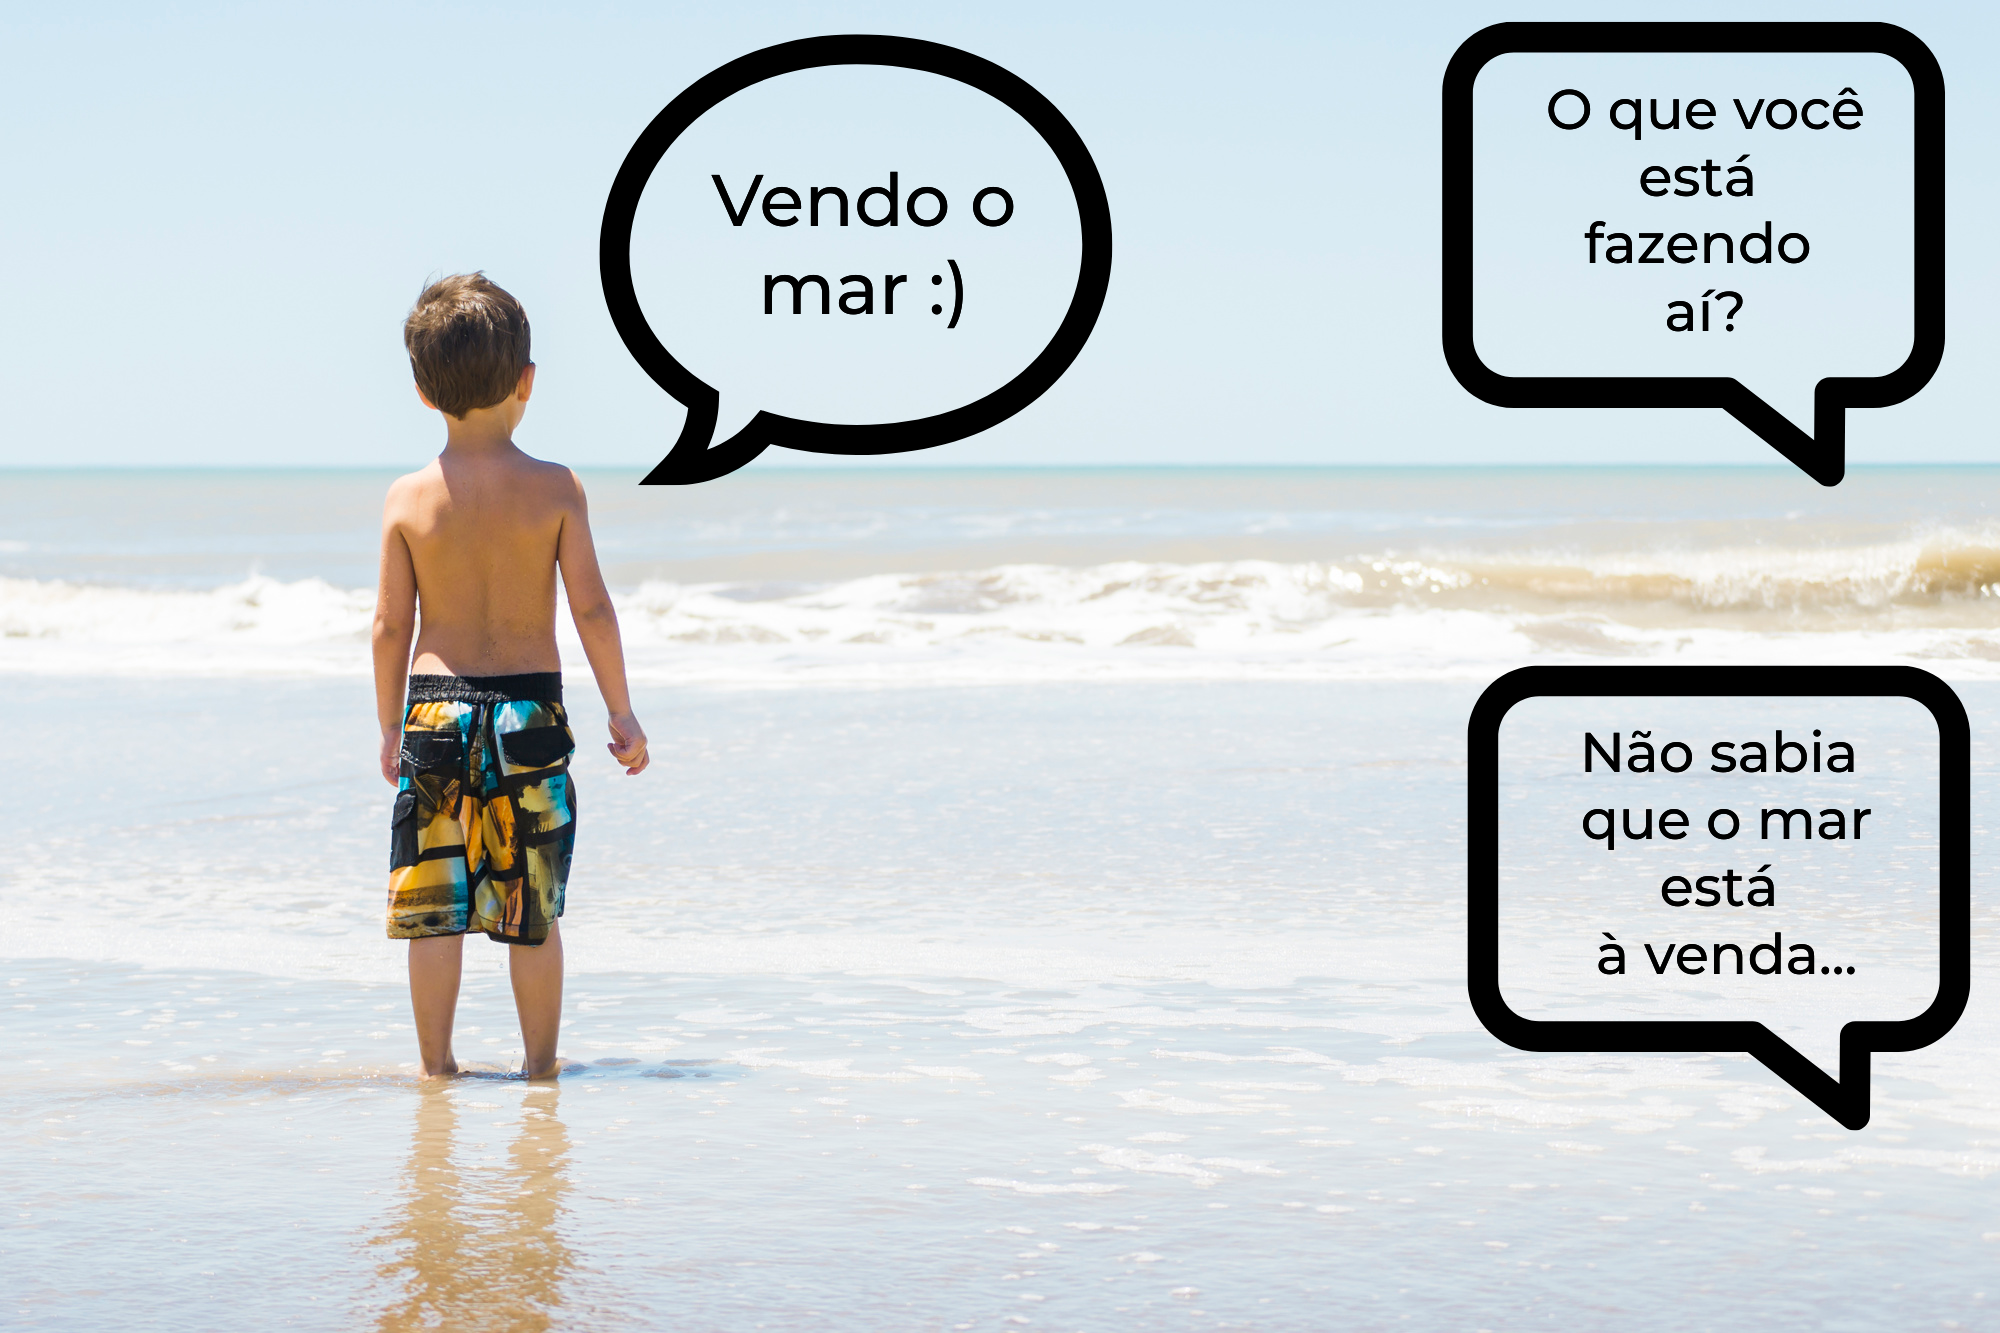
\includegraphics[width=\textwidth]{./imgSAEB_7_POR/media/image4.png}
\end{figure}

\num{1} No meme acima pode-se perceber que o humor está presente. Qual  palavra está sendo usada para produzir esse efeito?

\reduline{A forma verbal ``vendo'' é utilizada para obter o efeito do 
humor.\hfill} 

\num{2} Por que o uso dessa palavra produz efeito de humor?

\reduline{No contexto, a palavra ``vendo'' pode ter assumir
sentidos diferentes, que causam o efeito de humor.\hfill}

\num{3} Quais as possíveis interpretações da palavra usada para produzir
efeito de humor no meme?

\reduline{A forma verbal ``vendo'' é entendida pela pessoa que faz a pergunta 
como primeira pessoa do singular do presente do indicativo do verbo 
\textit{vender}, isto é: para ele, a criança \textit{está vendendo} o pôr do sol. 
Ela, por sua vez, quer dizer que está 
\textit{observando} o pôr do sol; neste sentido, ``vendo'' é gerúndio do
verbo \textit{ver}.\hfill} 

\num{4} Em qual sentido a forma verbal ``vendo'' está sendo usada pela
criança?

\reduline{A criança quer dizer que está 
\textit{observando} o pôr do sol; neste sentido, ``vendo'' é gerúndio do
verbo \textit{ver}.\hfill} 

\num{5} Em qual sentido está sendo compreendida a forma verbal ``vendo''
pela pessoa que faz a pergunta?

\reduline{A forma verbal ``vendo'' é entendida pela pessoa que faz a 
pergunta como primeira pessoa do singular do presente do indicativo 
do verbo \textit{vender}, isto é: para quem faz a pergunta, a criança 
\textit{está vendendo} o pôr do sol.\hfill}

\num{6} Em qual balão a questão das diferentes interpretações da 
forma verbal se esclarece?

\reduline{As diferentes interpretações da forma verbal se esclarecem 
no último balão.\hfill}

Analise a imagem abaixo e responda às questões de 7 a 10. 

\begin{figure}[h!]
\centering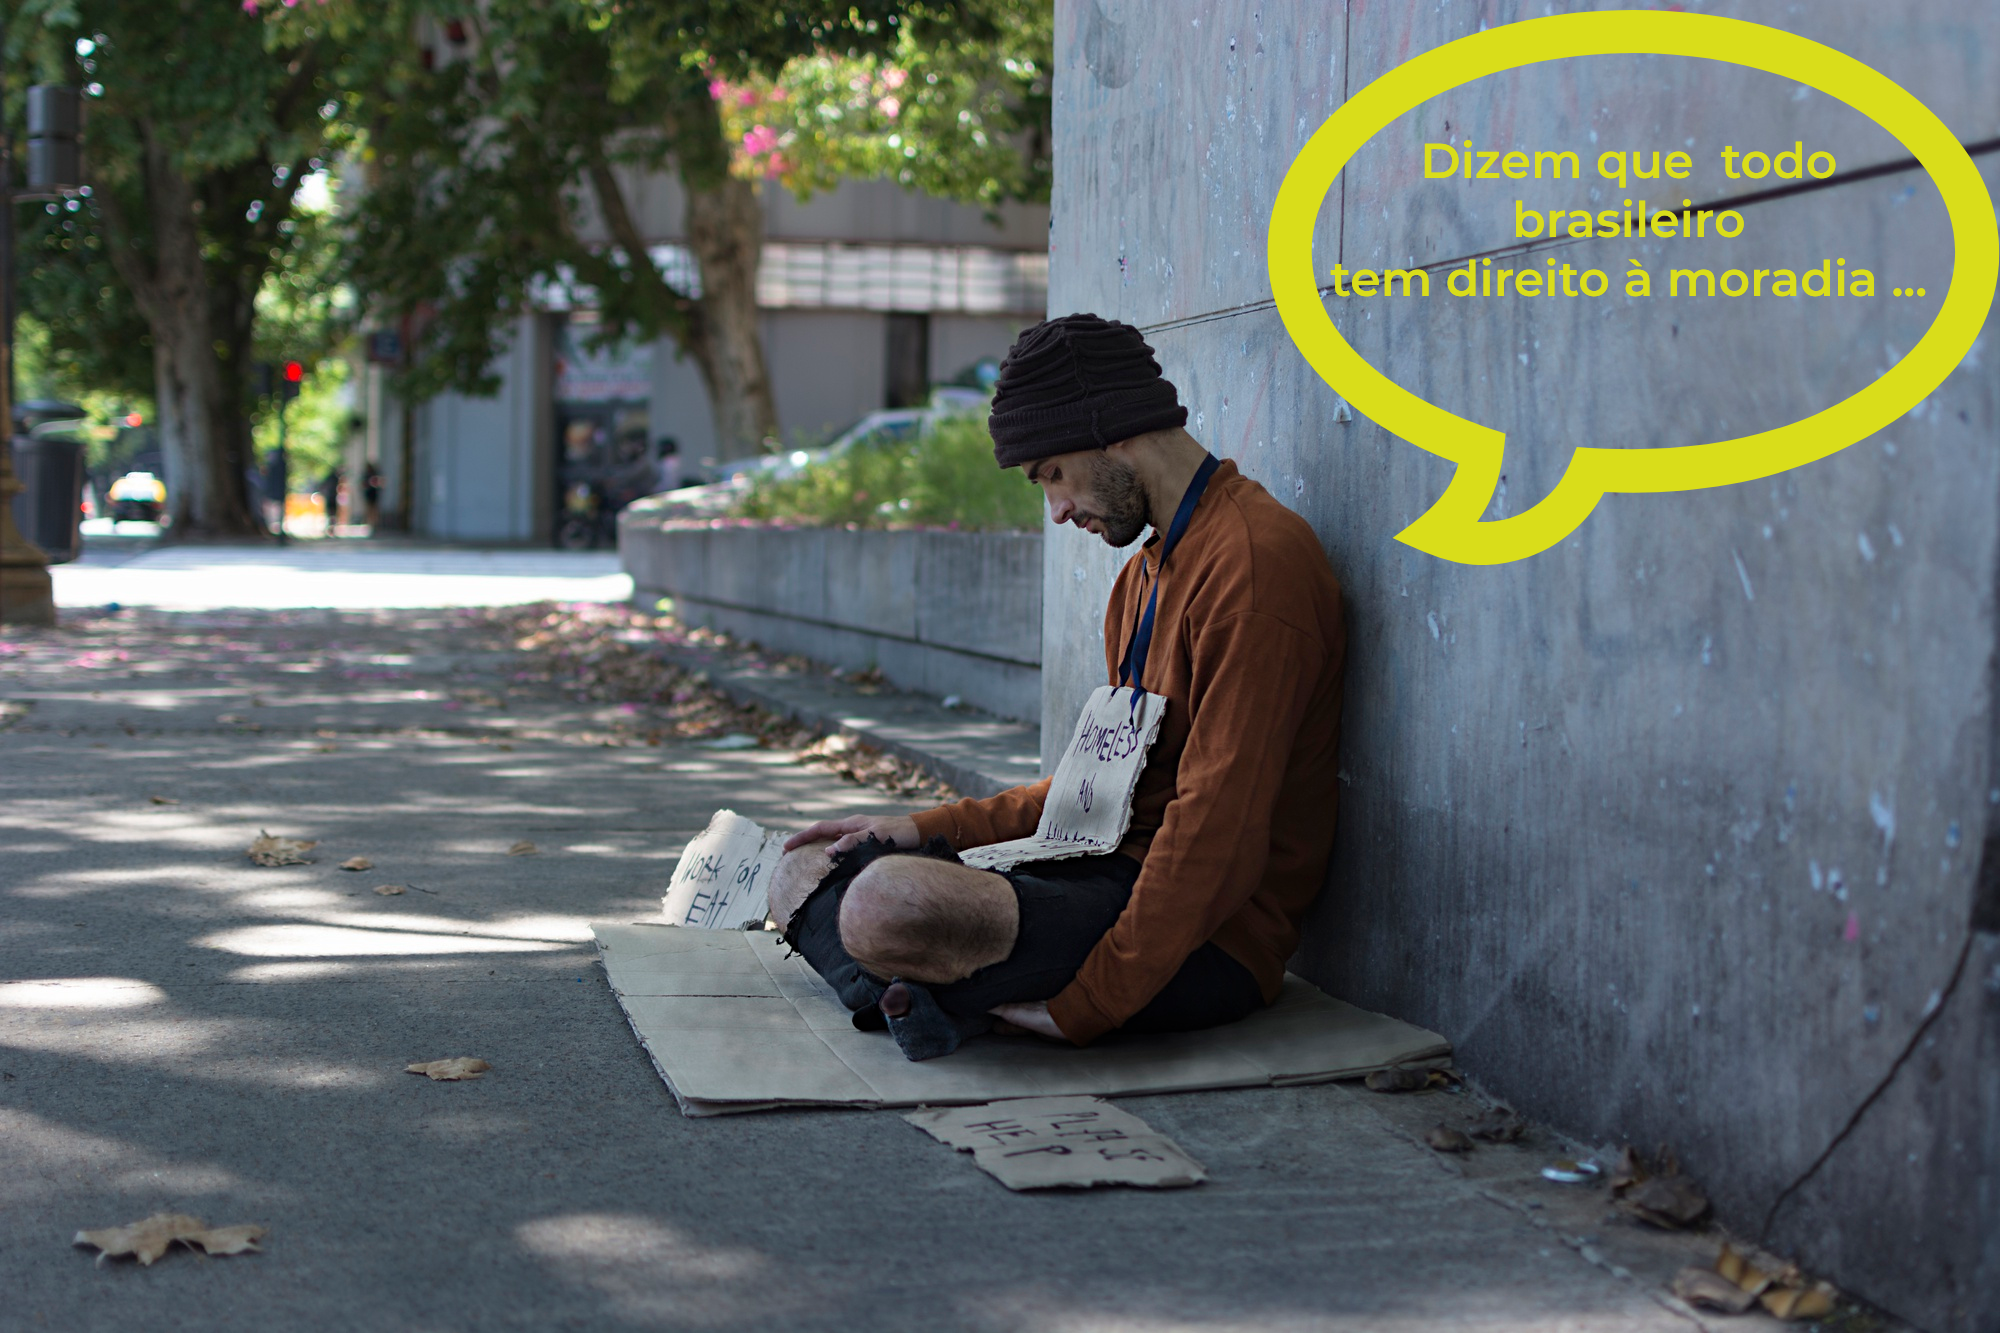
\includegraphics[width=5in]{./imgSAEB_7_POR/media/image5.png}
\end{figure}

\num{7} Considerando a imagem, é possível
inferir que a fala do morador em situação de rua alude a um importante
documento da democracia brasileira. Que livro é
esse?

\reduline{É possível inferir que a fala do morador em situação de rua
alude à Constituição Federal de 1988.\hfill}

\num{8} Qual a função deste documento e o que ele pretende garantir?

\reduline{A Constitução Federal trata das questões mais importantes 
para a manutenção da democracia e pretende esclarecer os direitos 
e deveres de todos os âmbitos da sociedade.\hfill}

\num{9} Qual o efeito de sentido obtido por meio do meme? 

\reduline{O efeito de sentido obtido por meio do meme é a ironia.\hfill}

\num{10} De que forma a imagem se articula com o texto para produzir
o efeito de sentido?

\reduline{No meme, uma pessoa em situação de rua reflete sobre um dos direitos 
fundamentais garantidos pela Constituição Federal de 1988: o direito à
moradia. A \textit{declaração} desse direito é rigorosamente oposta à 
\textit{situação concreta} em que se encontra o morador. Essa oposição
compõe a ironia, que consiste em dizer o inverso do que se quer afirmar.
Evidentemente, o autor do meme pretende evidenciar o contraste entre discurso e
prática, isto é, entre a afirmação dos direitos na Constituição de 1988 e a 
desigualdade social.\hfill} 

\section{Treino}

\num{1} Leia o trecho abaixo para responder à questão. 

\begin{myquote}

Há meio século, os escravos fugiam com frequência. Eram muitos, e nem todos
gostavam da escravidão. Sucedia ocasionalmente apanharem pancada, e nem todos
gostavam de apanhar pancada. Grande parte era apenas repreendida; havia alguém de
casa que servia de padrinho, e o mesmo dono não era mau; além disso, o sentimento da
propriedade moderava a ação, porque dinheiro também dói. A fuga repetia-se,
entretanto. Casos houve, ainda que raros, em que o escravo de contrabando, apenas
comprado no Valongo, deitava a correr, sem conhecer as ruas da cidade.

\end{myquote}

\fonte{Machado de Assis. Pai contra Mãe. Disponível em: 
http://www.dominiopublico.gov.br/download/texto/bv000245.pdf.
Acesso em: 22 mai. 2023.}

No fragmento do conto ``Pai contra Mãe'', o narrador de Machado de Assis faz a crítica
à escravidão brasileira por meio de:

\begin{escolha}

  \item repetições que resultam em ironia.
  
  \item relato objetivo da realidade.
  
  \item observações nostálgicas. 
  
  \item valorização dos escravizados. 

\end{escolha}


\num{2} Observe a imagem abaixo para responder à questão. 

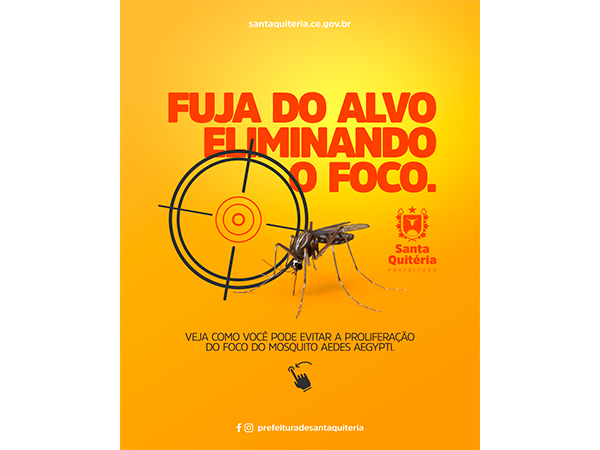
\includegraphics[width=5.90551in,height=4.43056in]{./imgSAEB_7_POR/media/image6.png}

\fonte{Prefeitura de Santa Quitéria. Dicas de como evitar a proliferação 
do foco do mosquito Aedes Aegypti. Disponível em: 
https://www.santaquiteria.ce.gov.br/informa.php?id=1018.
Acesso em: 22 mai. 2023.}

Na imagem acima observa-se uma campanha para evitar a proliferação do
mosquito da dengue. A escolha das palavras e imagens tem como objetivo
sensibilizar a população. Assinale a alternativa que contém as palavras
usadas para a produção de efeito de sentido na campanha. 

\begin{escolha}
  
  \item Proliferação e foco.
  
  \item Veja e evitar.
  
  \item Fuja e elimine.
  
  \item Alvo e foco. 

\end{escolha}

\num{3} Leia o texto abaixo para responder à questão.


\includegraphics[width=\textwidth]{./imgSAEB_7_POR/media/image7.png}

A respeito do meme acima, pode-se afirmar que

\begin{escolha}
    
    \item ironiza a educação por meio do duplo sentido da palavra ``casa''.
    
    \item critica a falta de moradia com o uso da palavra ``casa''.
    
    \item contém propaganda subliminar em benefício da construção de apartamentos.
    
    \item questiona a qualidade de vida dos moradores de apartamentos.

\end{escolha}

\chapter{Parcialidade nos textos jornalísticos}
\markboth{Módulo 7}{}

\section{Habilidades do SAEB}

\begin{itemize}

  \item Analisar marcas de parcialidade em textos jornalísticos.

  \item Avaliar diferentes graus de parcialidade em textos jornalísticos.

  \item Avaliar a fidedignidade de informações sobre um mesmo fato divulgado 
  em diferentes veículos e mídias.

\end{itemize}

\subsection{Habilidades da BNCC}

\begin{itemize}

  \item EF07LP02, EF67LP03, EF67LP04.

\end{itemize}

\conteudo{A função ideal do jornalismo é informar de forma imparcial e objetiva
fatos e notícias para oferecer informações e ferramentas para a
formação de opinião. No entanto, nem sempre é possível separar os fatos
das opiniões, pois todo texto, em alguma medida, é produzido a partir
das perspectivas pessoais do autor ou do veículo de comunicação que o
divulga. Por isso, é importante que os leitores aprendam a analisar
marcas de parcialidade em textos jornalísticos, a fim de avaliar o grau
de confiabilidade das informações que estão recebendo.

Uma das formas de identificar as marcas de parcialidade em textos
jornalísticos é perceber o conjunto de valores expressos pelo uso de
adjetivos, advérbios e na forma como são construídos os argumentos nos
textos de divulgação de notícias e acontecimentos. Também a escolha de
fontes e a seleção editorial dos assuntos e temas a serem tratados podem
indicar interesses e, portanto, certo grau de parcialidade. A escolha
dos pontos de vista expressos em uma notícia ou reportagem revela muito
sobre as intenções do autor ou do veículo que divulga o texto. Sendo
assim, comparar fontes e analisar de forma atenta os contextos em que as
informações são divulgadas em cada veículo de informação pode ser uma
forma eficaz de avaliar a confiabilidade e fidedignidade de determinada
notícia ou reportagem, porque a linha editorial e a relação dos
veículos de comunicação com empresas e grupos políticos ou econômicos
podem revelar possíveis interesses e pontos de vista. Portanto, aprender
a avaliar tais marcas de parcialidade e comparar diferentes formas de
divulgação de notícias em diversos veículos e texto é uma habilidade
importante para que o leitor possa formar uma opinião de forma reflexiva
e autônoma.}

% \coment{Professor(a), faça um exercício de reflexão com os estudantes,
% questionando como percebem os traços e interesses presentes em algumas
% manchetes, e chamadas. Chame a atenção para veículos sensacionalistas,
% para determinados temas e assuntos abordados e veiculados com a intenção
% de gerar polêmicas, discussões ou busca de soluções. Converse com os
% estudantes sobre os diversos tipos de textos jornalísticos e estimule-os
% a refletir sobre como percebem as marcas de parcialidade. Instrua-os a
% pesquisar e questionar os veículos de comunicação trazendo para a
% discussão quais podem ser os interesses por trás dos recursos e
% elementos multissemióticos presentes nas informações que consomem. Cite
% a monetização de determinados conteúdos, explique como é importante
% analisar quem são os financiadores e quais as propagandas e empresas
% relacionadas aos veículos de informação que conhecem.}

\section{Atividades}

Analise as duas notícias abaixo e responda às questões.

\begin{myquote}

\textbf{Texto I}: Cinco desafios para a economia mundial em 2023

Se 2022 foi um ano difícil para a economia global, 2023 promete ser
ainda pior, com uma recessão a caminho.

Espera-se que 2023 seja o terceiro ano com o pior crescimento econômico
global neste século, atrás de 2009, quando a crise financeira global
causou a Grande Recessão, e 2020, quando os lockdowns da covid-19
virtualmente paralisaram a economia global.

Analistas esperam que as principais economias do mundo, incluindo os
Estados Unidos e o Reino Unido, assim como a zona do euro, entrem em
recessão este ano, já que os bancos centrais continuam aumentando as
taxas de juros para moderar a demanda por bens de consumo e serviços, em
um esforço para conter a inflação. 

\fonte{Ashutosh Pandey. DW. Cinco desafios para a economia mundial em 2023.
Disponível em: https://www.dw.com/pt-br/cinco-desafios-para-a-economia-mundial-em-2023/a-64264182.
Acesso em: 22 mai. 2023. com adaptações.}

\end{myquote}

\begin{myquote}

\textbf{Texto II}:Por que a inflação mundial deve cair em 2023 (e por que a
notícia não é tão boa)

Provavelmente o pior em termos de inflação já passou.

Pelo menos este é o consenso entre os economistas e as principais
organizações econômicas como o Fundo Monetário Internacional (FMI) ou o
Banco Mundial depois que a maioria dos países do mundo experimentou, em
2022, aumentos de preços não vistos em quatro décadas.

Não há dúvida de que a inflação continuará a pesar no bolso de milhões
de cidadãos em 2023, mas deve registrar uma queda lenta nos próximos 12
meses.

Quando esse período terminar, o FMI espera que a inflação mundial caia
para 4,7\%, pouco menos da metade do nível atual. 

\end{myquote}

\fonte{Cristina J. Orgaz. BBC News Brasil. Por que a inflação mundial deve cair em 2023 (e por que a notícia não é tão boa). 
Disponível em: https://www.bbc.com/portuguese/internacional-64145595.
Acesso em: 22 mai. 2023.}

\num{1} Qual é o fato central relatado nas notícias?

\reduline{O fato central das duas notícias é a crise econômica de 2023.\hfill}

\num{2} Quais são as semelhanças entre os fatos noticiados sobre o tema?

\reduline{As duas notícias tratam da recessão e da influência da queda da
inflação na crise econômica mundial.\hfill}

\num{3} Quais são as diferenças entre os fatos noticiados sobre o tema?

\reduline{No primeiro texto, o autor prevê, em 2023, a continuidade da crise
econômica. O autor segundo sinaliza, por sua vez, uma queda na inflação.\hfill} 

\num{4} Em qual das duas notícias a crise mundial é tratada com mais otimismo?
Copie do texto um trecho que justifique sua resposta.

\reduline{O Texto II é mais otimista, como se verifica no trecho 
``Provavelmente o pior em termos de inflação já passou''.\hfill}

\num{5} Na tabela abaixo, relacione os títulos numerados à esquerda
com as linhas finas à direita.

\begin{table}[h!]
\begin{tabular}{|c|c|c|c|}
\hline
\textbf{} & \textbf{Título} & \textbf{} & \textbf{Linha fina} \\ \hline
\textbf{1} & \begin{tabular}[c]{@{}c@{}}Estudiosos alertam para os riscos de doenças \\ cardiovasculares e o sedentarismo\end{tabular} & \rosa{1} & \begin{tabular}[c]{@{}c@{}}Análise de hábitos de pacientes com problemas cardiovasculares \\ traz novas informações sobre como prevenir doenças crônicas\end{tabular} \\ \hline
\textbf{2} & Casos de dengue preocupam secretarias de saúde & \rosa{3} & \begin{tabular}[c]{@{}c@{}}Associação brasileira de pediatria publica estudo sobre os impactos\\  dos jogos e redes sociais na vida de adolescentes\end{tabular} \\ \hline
\textbf{3} & \begin{tabular}[c]{@{}c@{}}O perigo está em casa: Pediatras alertam sobre o uso \\ excessivo de telas por crianças e adolescentes\end{tabular} & \rosa{4} & \begin{tabular}[c]{@{}c@{}}Ministério da saúde lança cartilha para informar a população \\ sobre as formas de contágio da doença\end{tabular} \\ \hline
\textbf{4} & Covid-19: Informar para proteger & \rosa{2} & \begin{tabular}[c]{@{}c@{}}Alerta foi dado às secretarias de saúde de todo país, especialmente \\ nas regiões em que se inicia o período de chuvas\end{tabular} \\ \hline
\end{tabular}
\end{table}
%Gabarito \coment{1, 3, 4, 2}

\num{6} Sobre a parcialidade dos textos jornalísticos, assinale V para as
afirmações verdadeiras e F para as afirmações falsas na tabela abaixo.

\begin{table}[h!]
\begin{tabular}{|c|c|}
\hline
\textbf{\begin{tabular}[c]{@{}c@{}}Verdeiro (V) \\ ou Falso (F)?\end{tabular}} & \textbf{Afirmações} \\ \hline
\rosa{V} & \begin{tabular}[c]{@{}c@{}}A imparcialidade no jornalismo é importante pois promove \\ a formação de opinião a partir dos fatos apresentados na reportagem\end{tabular} \\ \hline
\rosa{F} & \begin{tabular}[c]{@{}c@{}}O princípio da imparcialidade no jornalismo significa que o jornalista \\ não deve apresentar os diferentes pontos de vista e deixar que o público \\ forme sua própria opinião\end{tabular} \\ \hline
\rosa{V} & \begin{tabular}[c]{@{}c@{}}A imparcialidade no jornalismo pode levar a erros de interpretação e \\ compreensão dos fatos por parte do público, prejudicando a credibilidade da reportagem do jornalista\end{tabular} \\ \hline
\rosa{V} & \begin{tabular}[c]{@{}c@{}}A falta de apresentação de fontes e dados confiáveis pode ser uma \\ característica de parcialidade por parte do jornalista ou do veículo de \\ comunicação colocando em dúvida a qualidade das notícias veiculadas\end{tabular} \\ \hline
\end{tabular}
\end{table}

%\coment{V, F, V, V}

\num{7} Leia os exemplos abaixo e sublinhe as marcas de parcialidade:

\begin{escolha}

  \item Polícia age com violência contra manifestantes pacíficos.

  \item Deputado faz discurso inflamado em defesa dos direitos dos
trabalhadores.

  \item Falas preconceituosas de senadores exibem a impunidade da classe
política no Brasil.

\end{escolha}

% \coment{a) Polícia age com \uline{violência} contra manifestantes
% \uline{pacíficos}.

% b) Deputado faz discurso \uline{inflamado} em defesa dos direitos dos
% trabalhadores.

% c) Falas \uline{preconceituosas} de senadores exibem a
% \uline{impunidade} da classe política no Brasil.}

\num{8} Quais aspectos devem ser levados em conta para questionar a
parcialidade ou imparcialidade de uma notícia

\reduline{Os aspectos que devem ser levados em conta são: a exposição de
mais de um ponto de vista sobre o mesmo tema, a citação de dados e 
pesquisas de fontes confiáveis e o uso ou não de adjetivos que qualifiquem
os fatos apresentados. É importante também a checagem da veracidade dos 
dados apresentados e o questionamento sobre os contextos em que ocorrem os
fatos e se há interesses políticos ou econômicos por parte do veículo de
comunicação que divulga a notícia.\hfill}

\num{9} Analise as duas afirmações a seguir e responda qual das duas apresenta
maior grau de parcialidade. Justifique sua resposta

\begin{itemize}
 
 \item Policiamento nas cidades não gera mais segurança, é o que afirmam
especialistas

  \item Policiamento nas cidades é a principal medida de segurança anunciada pela prefeitura.

\end{itemize}

\reduline{A primeira afirmação apresenta maior grau de parcialidade, pois
apresenta uma afirmação categórica amparada em afirmação de especialistas. 
A segunda é uma sentença menos parcial, embora contenha o adjetivo ``principal'' 
para referir-se ao fato noticiado.\hfill}

\num{10} De que forma a apresentação de imagens, gráficos e tabelas auxilia 
na formação de opinião de leitores?

\reduline{A apresentação de imagens, gráficos e tabelas confere 
clareza e credibilidade à notícia, pois esses recursos podem ser
interpretados, questionados e verificados.}

\section{Treino}

\num{1} Sabendo da importância de aprender a analisar traços de parcialidade em
textos jornalísticos, assinale a alternativa que contém um recurso por meio
do qual o texto jornalístico tende a ser mais parcial.

\begin{escolha}

  \item Entrevistas com especialistas no assunto abordado.
  \item Diferentes pontos de vista sobre o mesmo assunto.
  \item Adjetivos valorativos para descrever pessoas ou eventos.
  \item Fatos e fontes citadas rigorosamente. 

\end{escolha}

\num{2} Leia o trecho abaixo e o gráfico que segue para responder à questão.

Não estamos no caminho certo para atingir as metas de mudança
climática. Se somarmos todas as promessas para reduzir emissões de gases
que provocam efeito estufa pelos países que assinaram o Acordo de Paris,
o mundo ainda esquentaria em mais de 3°C até o fim deste século.

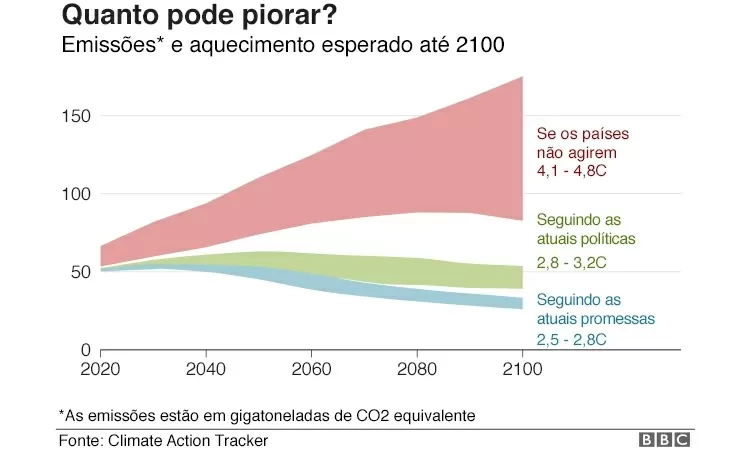
\includegraphics[width=5.90551in,height=3.56944in]{./imgSAEB_7_POR/media/image8.png}

\fonte{BBC News Brasil. Aquecimento global: 7 gráficos que mostram em que ponto estamos. Disponível em: https://www.bbc.com/portuguese/geral-46424720. 
Acesso em: 22 mai. 2023.}

Assinale a alternativa que contém o principal recurso para obter o efeito da 
confiabilidade da notícia:

\begin{escolha}

  \item a opinião do jornalista.
  
  \item a oposição ao Acordo de Paris.
  
  \item o uso de gráficos de pesquisas.
  
  \item o uso de expressões sensibilizadoras.

\end{escolha}

\num{3} Leia o texto abaixo para responder à questão.

\begin{myquote}

\textbf{Após três anos sem reajuste, tarifa de ônibus é corrigida abaixo da
inflação do período}

A partir de 1° de janeiro de 2023, o transporte coletivo urbano de
Joinville passará a operar com os valores de R\$5,25 para a tarifa
antecipada e R\$5,50 para a tarifa embarcada (modalidade utilizada por
apenas 5\% dos passageiros). O reajuste representa aproximadamente
metade do percentual de inflação dos últimos três anos, período no qual
a tarifa não foi corrigida.

\end{myquote}

\fonte{Prefeitura de Joinville. Após três anos sem reajuste, tarifa de ônibus é 
corrigida abaixo da inflação do período. Disponível em: https://www.joinville.sc.gov.br/noticias/apos-tres-anos-sem-reajuste-tarifa-de-onibus-e-corrigida-abaixo-da-inflacao-do-periodo/
Acesso em: 22 mai. 2023.}

A matéria apresenta grau de parcialidade, pois apresenta:

\begin{escolha}
  
  \item justificativa para o aumento desde o título.
  
  \item informações precisas sobre a data do ocorrido
  
  \item informações sobre os valores da passagem
  
  \item dados sobre os usuários do transporte público na cidade

\end{escolha}


\chapter{Recursos de modalização e argumentação}
\markboth{Módulo 8}{}

\section{Habilidades do SAEB}

\begin{itemize}

  \item Identificar os recursos de modalização em textos diversos.

  \item Analisar os efeitos de sentido dos tempos, modos e/ou vozes 
verbais com base no gênero textual e na intenção comunicativa.

  \item Analisar os efeitos de sentido produzidos pelo uso de modalizadores em textos diversos.

\end{itemize}

\subsection{Habilidades da BNCC}

\begin{itemize}

  \item EF69LP04, EF69LP28, EF07LP14.

\end{itemize}

\conteudo{A capacidade de identificar e compreender os recursos de modalização
presentes em diferentes tipos de texto é fundamental para uma
comunicação eficiente e coerente. A modalização envolve o uso de
recursos linguísticos para expressar atitudes e opiniões do emissor em
relação ao conteúdo abordado. Esses recursos podem estar
presentes nas formas de uso de modos e vozes verbais, além de adjetivos e advérbios.

A análise dos efeitos de sentido produzidos pelos recursos de
modalização em diferentes gêneros textuais e intenções comunicativas é
fundamental para identificar as influências destes recursos na percepção
e compreensão do conteúdo pelo receptor.

Os recursos de modalização permitem que o emissor expresse suas
opiniões, transmita suas expectativas, faça indicações, influenciando
assim na percepção dos leitores. Dentre os principais recursos
de modalização, encontram-se os tempos verbais, os modos verbais, as
vozes verbais e os modalizadores, que podem reformar graus de
probabilidade, certeza, necessidade e urgência.

Portanto, compreender e utilizar os recursos de modalização de forma
adequada é essencial para produzir textos claros, coerentes e
persuasivos, adaptando a linguagem ao tipo de público alvo e ao contexto
em que são emitidos. Além disso, a análise crítica desses recursos
permite que o leitor compreenda as intenções do emissor e as influências
que podem estar presentes no conteúdo do texto.}

% \coment{Professor(a), estimule os estudantes a lembrarem do uso destes recursos
% em exemplos conhecidos e práticos tais como campanhas de conscientização
% ou publicitárias. Retome os recursos de modalização presentes em
% diversos gêneros textuais já estudados demonstrando as diferenças de
% interpretação e sentido possíveis para os usos de tempos e modos
% verbais, tais como infinitivo e imperativo, das vozes do texto, dos
% discursos diretos e indiretos e do uso de advérbios que qualificam as
% ações com advérbios que indicam urgência, condições, sugestões,
% obrigatoriedade, etc.}

\section{Atividades}


\includegraphics[width=2.85536in,height=2.85536in]{./imgSAEB_7_POR/media/image9.png}

% \fonte{https://itajuba.mg.gov.br/secretariaspmi/semdes/nao_desvie_o_olhar/}{\uline{https://itajuba.mg.gov.br/secretariaspmi/semdes/nao\_desvie\_o\_olhar/}}.
% Acesso em: 18 de abr de 2023

\fonte{itajuba.mg.gov.br}


\num{1} Retire da imagem acima os elementos modalizadores que produzem o sentido de instrução.

\reduline{As formas verbais no imperativo produzem o sentido de instrução no texto.\hfill}

\num{2} De que forma o uso desses recursos sensibiliza o leitor?

\reduline{As formas verbais no imperativo apelam para a responsabilidade individual do leitor quanto
à violência contra crianças e adolescentes.\hfill}

\num{3} Observe as informações contidas no cartaz e explique qual é a ação
recomendada ao tomar conhecimento de casos de violência contra crianças e adolescentes.

\reduline{Ligar para o telefone indicado e denunciar a violência contra crianças e adolescentes é 
a ação recomendada.\hfill}

\num{4} Relacione as colunas de expressões com seus respectivos efeitos de sentido:

% Please add the following required packages to your document preamble:
% \usepackage[table,xcdraw]{xcolor}
% If you use beamer only pass "xcolor=table" option, i.e. \documentclass[xcolor=table]{beamer}

% REVER
% \begin{table}[h!]
% \begin{tabular}{|cc|cc|}
% \hline
% \rowcolor[HTML]{FD6864} 
% \multicolumn{2}{|c|}{\cellcolor[HTML]{FD6864}\textbf{Efeito de sentido}} & \multicolumn{2}{c|}{\cellcolor[HTML]{FD6864}\textbf{Expressão}} \\ \hline
% \multicolumn{1}{|c|}{\textbf{I}} & Obrigação & \multicolumn{1}{c|}{} & felizmente \\ \hline
% \rowcolor[HTML]{FFCCC9} 
% \multicolumn{1}{|c|}{\cellcolor[HTML]{FFCCC9}\textbf{II}} & Apreciação & \multicolumn{1}{c|}{\cellcolor[HTML]{FFCCC9}} & é dever de todos \\ \hline
% \multicolumn{1}{|c|}{\textbf{III}} & Possibilidade & \multicolumn{1}{c|}{} & é impossível \\ \hline
% \rowcolor[HTML]{FFCCC9} 
% \multicolumn{1}{|c|}{\cellcolor[HTML]{FFCCC9}\textbf{IV}} & Certeza & \multicolumn{1}{c|}{\cellcolor[HTML]{FFCCC9}} & provavelmente \\ \hline
% \end{tabular}
% \end{table}

% \coment{II, I, IV, III}

Leia a afirmação abaixo e responda à questão.

\begin{myquote}

\textbf{Certamente}, com a implementação dos projetos de mobilidade
urbana, as pessoas passarão a ter mais qualidade de vida e mais
liberdade para explorar e ocupar a cidade.

\end{myquote}

\num{5} Qual sentido a palavra destacada pretende expressar?

\reduline{A palavra destacada pretende expressar certeza sobre as consequências da melhoria da
mobilidade urbana.\hfill}

Observe a campanha a seguir e responda:


\includegraphics[width=5.90551in,height=1.47222in]{./imgSAEB_7_POR/media/image10.png}


\fonte{Agência de Transporte do Estado de São Paulo.}

% \fonte{Agência de Transporte do Estado de São Paulo. #FocaNaVida. Disponível em:
% http://www.artesp.sp.gov.br/Style\%20Library/extranet/campanha-interna.aspx?id=1
% Acesso em: 22 mai. 2023.}

\num{6} Qual a ideia transmitida pela conjunção ``se'' na frase, 
``Nesse carnaval se beber, não dirija''?

\reduline{A conjunção ``se'', na frase analisada, é condicional, ou seja, é por meio dela que 
se propõe a condição expressa na frase: caso o leitor tenha bebido, não deve dirigir.\hfill} 

\num{7} Ainda sobre a campanha acima, assinale verdadeiro ou falso na tabela para as afirmações a seguir.

\begin{table}[h!]
\begin{tabular}{|c|c|}
\hline
\textbf{\begin{tabular}[c]{@{}c@{}}Verdadeiro (V)\\ ou Falso (F)?\end{tabular}} & \textbf{Afirmações} \\ \hline
\rosa{V} & a campanha sugere que não se deve dirigir após beber \\ \hline
\rosa{F} & a campanha sugere que as pessoas não devem beber durante o carnaval \\ \hline
\rosa{F} & a campanha orienta os foliões a não dirigir no carnaval \\ \hline
\rosa{F} & a campanha pretende alertar sobre a violência no trânsito \\ \hline
\end{tabular}
\end{table}



%Gabarito \coment {V, F, F, F}

\num{8} Leia os enunciados e enumere as proposições na tabela.

\begin{table}[h!]
\begin{tabular}{|c|l|c|l|}
\hline
\textbf{} & \multicolumn{1}{c|}{\textbf{Enunciado}} & \textbf{} & \multicolumn{1}{c|}{\textbf{Efeito}} \\ \hline
\textbf{1} & É necessária a presença de um acompanhante & \rosa{2} & Expressa proibição \\ \hline
\textbf{2} & É proibida a entrada de acompanhante & \rosa{1} & Expressa obrigatoriedade \\ \hline
\textbf{3} & É permitida a entrada de um acompanhante & \rosa{3} & Expressa permissão \\ \hline
\end{tabular}
\end{table}

%Gabarito: \coment{2, 1, 3}

%Leia tirinha abaixo para responder à questão.

%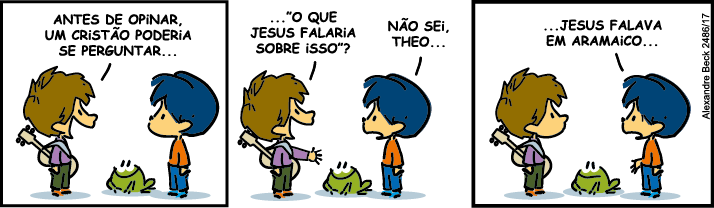
\includegraphics[width=5.90551in,height=1.72222in]{./imgSAEB_7_POR/media/image11.png}

%\fonte{https://tirasarmandinho.tumblr.com/}{\uline{https://tirasarmandinho.tumblr.com/}}
%Acesso em 19 de Abr de 2023

%\num{9}
%Qual é a confusão comunicativa presente na tirinha?
%
%
%A confusão se dá pois os personagens entendem o verbo falar em sentidos diferentes

%\num{10} Qual o sentido do verbo falar no segundo quadrinho? Escreva um sinônimo.

%O verbo falar no segundo quadrinho se refere a opinião, e poderia ser
%substituído por dizer ou pensar. Pensaria, diria.

\section{Treino}

\num{1} Leia o texto abaixo para responder à questão.

\begin{myquote}

Antes da pandemia causada pelo novo coronavírus, era quase impensável
ver grande parte da população usando máscaras de proteção na rua.
Contudo a situação mudou, principalmente após o governo do estado tornar
seu uso obrigatório. Mesmo assim, ainda há dúvidas de parte da população
quanto à necessidade e ao benefício do seu uso.

\end{myquote}

% \fonte{Secretaria de Estado de Saúde de Minas Gerais. Notas de Recomendação: Covid 19.
% Disponível em: https://coronavirus.saude.mg.gov.br/blog/101-mascaras-e-covid-19.
% Acesso em: 22 mai. 2023.}
\fonte{Secretaria de Estado de Saúde de Minas Gerais.}

No contexto em que se insere, a expressão ``mesmo assim'' expressa oposição entre:


\begin{escolha}

  \item o período anterior e o posterior à pandemia do coronavírus.

  \item a alta adesão da população ao uso de máscaras e a obrigatoriedade de usá-las.

  \item a obrigatoriedade do uso de máscaras e a atitude da população quanto a essa medida.

  \item grande parte da população utilizando máscaras de proteção e a minoria em dúvida.

\end{escolha}


\num{2} Leia o texto abaixo para responder à questão. 

\begin{myquote}

Carlos observava toda aquela pompa ao seu redor. Ele mesmo estava de passagem,
era um turista simples, brasileiro comum, passeando a custo do dinheiro suado, 
guardado todo mês, para conhecer aquela terra estrangeira e faustosa, cheia de 
gente milionária e bem vestida, cheirosa e fútil. Como deve ser triste depender
do luxo para ser feliz! --- pensava ele.     

\end{myquote}

\fonte{Rogério Duarte. Viagens pela terra dos outros. Saíra Editorial. no prelo.}

Na frase ``Como \textbf{deve} ser triste depender do luxo para ser feliz!'', 
a forma verbal destacada expressa:



\begin{escolha}
  
  \item Obrigação
  
  \item Conselho
  
  \item Causa
  
  \item Possibilidade

\end{escolha}


\num{3} Analise o cartaz abaixo para responder à questão.


\includegraphics[width=5.90551in,height=4.29167in]{./imgSAEB_7_POR/media/image13.png}

\fonte{Ministério da Integração e do Desenvolvimento Regional. Consumo consciente da água 
é base para um futuro sustentável. Disponível em: https://www.gov.br/dnocs/pt-br/assuntos/noticias/consumo-consciente-da-agua-e-base-para-um-futuro-sustentavel.
Acesso em: 22 mai. 2023.}

O uso do gerúndio na campanha acima expressa:

\begin{escolha}

  \item ação contínua.
  \item ordem a ser acatada.
  \item sugestão a ser considerada.
  \item condição.

\end{escolha}


\chapter{Figuras de linguagem como estratégia argumentativa}
\markboth{Módulo 9}{}

\section{Habilidades do SAEB}

\begin{itemize}
  
  \item Analisar o uso de figuras de linguagem como estratégia argumentativa.

  \item Avaliar a eficácia das estratégias argumentativas em textos de diferentes gêneros.

\end{itemize}

\subsection{Habilidades da BNCC}

\begin{itemize}

  \item EF69LP17, EF67LP38.

\end{itemize}

\conteudo{A linguagem tem como principal objetivo a comunicação, portanto, é
impossível distinguir a linguagem da interação que ela provoca. Quanto
maior o domínio das ferramentas de linguagem por parte do autor, maior o
nível de interação e conexão será atingido com o leitor. Do outro lado,
quanto mais o leitor for capaz de reconhecer as ferramentas e recursos
de expressividade, melhor será sua experiência de leitura. Existem diversas 
maneiras de promover maior expressividade
das palavras e, assim, facilitar e potencializar a interação por meio
da comunicação. Dentre esses recursos estão as chamadas figuras de
linguagem. São formas de interação que podem trazer maior expressividade 
ao texto, seja ele escrito ou transmitido oralmente.

Cada figura de linguagem tem características próprias e pode ser
utilizada de diversas maneiras, de acordo com o objetivo do falante ou
do escritor, com a situação comunicativa e com o interlocutor. As
figuras de linguagem podem fazer alusão ao sentido figurado das palavras
e expressões, tratar com exagero para exacerbar características e
impressões ou contrapor palavras com sentidos antagônicos demonstrando
valores de forma implícita. Por essas características, as figuras de
linguagem são recursos comunicativos de grande utilidade, especialmente
para escrita de textos do campo artístico literário como letras de
música e poemas. Também podem apresentar-se como recurso de persuasão e
comunicação importante nos textos do campo jornalístico
midiático.

A \textbf{metáfora} é uma figura de linguagem utilizada para
estabelecer uma relação de semelhança e comparação entre dois termos
distintos. Um exemplo do uso da metáfora é a expressão ``sua vida era um
mar de rosas''. Nesse caso, a expressão ``mar de rosas'' não tem sentido
literal, mas figurado, pois se refere a algo agradável e
prazeroso e não ao mar em sentido literal.

A \textbf{metonímia}, por sua vez, é a figura de linguagem utilizada quando se
lança mão um termo para se referir a outro, com o qual ele mantém uma
relação de proximidade, contiguidade e pertencimento. Ou seja, dizer que
``a cidade se beneficiou com as obras de infraestrutura'' é utilizar a metonímia,
por meio da qual o termo ``a cidade'' se refere à população da cidade. A metonímia
tem o efeito de tornar a linguagem mais concisa e precisa, evitando a repetição de
termos e textos muito extensos. É uma forma de dinamizar a comunicação e
potencializar a capacidade comunicativa.

Por meio da \textbf{personificação} atribuem-se características humanas a animais
e objetos. A personificação tem o efeito de tornar a linguagem mais expressiva e 
poética, pois humaniza seres e fenômenos, produzindo alto grau de identificação do
leitor com a experiência, sensação ou impressão que se pretende comunicar.

Por fim, a \textbf{hipérbole} é a figura de linguagem que aumenta ou exagera
determinada característica como forma de expressão.}

% \coment{Professor(a) faça um levantamento dos conhecimentos prévios que os 
% estudantes já têm. Deixe que tragam
% exemplos e forneça mais informações sobre os conceitos, chamando a
% atenção para as possibilidades expressivas das figuras de linguagem.
% Mostre como o uso das figuras de linguagem podem ampliar os efeitos de
% sentido, em quaisquer gêneros textuais.}

\section{Atividades}

Leia os primeiros versos do Hino Nacional Brasileiro para responder às perguntas:

\begin{myquote} 

Ouviram do Ipiranga as margens plácidas
De um povo heroico o brado retumbante.

\end{myquote}

% \fonte{Joaquim Osório Duque Estrada. Hino Nacional Brasileiro. 
% Disponível em: https://www.planalto.gov.br/ccivil_03/constituicao/hino.htm.
% Acesso em: 22 mai. 2023.}

\fonte{Joaquim Osório Duque Estrada. Hino Nacional Brasileiro.}

\num{1} Coloque os versos e termos da oração na ordem direta para compreender 
melhor o sentido da frase. 

\reduline{As margens plácidas do Ipiranga ouviram o brado retumbante de um povo heroico.\hfill}

\num{2} Quais são as figuras de linguagem presentes nos dois primeiros versos do 
Hino Nacional Brasileiro? Justifique sua resposta.

\reduline{As figuras de linguagem são o hipérbato -- isto é, a inversão dos termos -- e a
personificação, atribuição de ações humanas (ouvir) a seres inanimados (as margens do 
Rio Ipiranga).\hfill}

\num{3} Qual é a figura de linguagem presente na frase ``Você tem um coração de pedra!''? 
Explique.

\reduline{Na frase ``Você tem um coração de pedra!'' existe metáfora. A metáfora é uma comparação
cujos termos são omitidos. Nesse caso, a comparação se dá por meio do elemento comum à pedra
e ao coração: sua \textit{dureza}.\hfill}

\num{4} Qual é a figura de linguagem presente na frase  ``Estou morrendo de medo''? Explique.

\reduline{Na frase  ``Estou morrendo de medo'' observa-se hipérbole, devido ao exagero.\hfill}

\num{5} Qual é a figura de linguagem presente na frase  ``As estrelas são os olhos dos deuses''?
Explique.

\reduline{Na frase ``As estrelas são os olhos dos deuses'' existe metáfora. A metáfora é uma comparação
cujos termos são omitidos. Nesse caso, a comparação se dá por meio do elemento comum às estrelas e 
e aos olhos: seu \textit{brilho e/ou sua posição privilegiada em relação aos homens}.\hfill}

\num{6} Sobre a hiperbole, assinale V para as afirmações verdadeiras e F para as falsas:

\begin{table}[h!]
\begin{tabular}{|c|c|}
\hline
\textbf{\begin{tabular}[c]{@{}c@{}}Verdadeiro (V) \\ ou\\ Falso (F)?\end{tabular}} &  \\ \hline
 & comparação entre palavras distintas, sem mostrar os termos dessa comparação \\ \hline
 & exagero do sentido de uma palavra ou expressão \\ \hline
 & substituição de uma palavra por outra \\ \hline
 & atribuição de características humanas a seres inanimados \\ \hline
\end{tabular}
\end{table}

%\coment{F, V, V, F}

Leia o texto abaixo para responder às questões.

\begin{myquote}

Na cordilheira que fica em cima do vale de Yyucay, em Cusco,
pode-se ouvir todos os sons. O vento sopra com sua bocarra;
a manhã, obrigada a se levantar sempre antes dos outros,
boceja morta de sono; os pássaros, seus eternos namorados,
acordam cantando ao ouvi-la se espreguiçar.

\end{myquote}

\fonte{Ana Rosa Abreu e outros autores. Alfabetização: livro do aluno. Vol.2: 
contos tradicionais, fábulas, lendas e mitos. Disponível em: 
http://www.dominiopublico.gov.br/download/texto/me001614.pdf.
Acesso em: 22 mai. 2023.}

\num{8} Copie do texto um exemplo de hipérbole.

\reduline{``bocarra''; ``boceja morta de sono''; ``eternos''.\hfill}

\num{10} Copie do texto um exemplo de personificação

\reduline{``O vento sopra com sua bocarra, os pássaros, seus eternos namorados,
acordam cantando ao ouvi-la se espreguiçar.''\hfill}

\section{Treino}

\num{1} Qual é a figura de linguagem presente na frase ``Brasil reforça postura de 
neutralidade e ganha espaço na geopolítica mundial''?

\begin{escolha}

  \item Personificação.
  
  \item Comparação.
  
  \item Hipérbole.
  
  \item Metonímia. 

\end{escolha}

\num{2} Leia um famosos trecho do romance \textit{Iracema}, de José de Alencar.

\begin{myquote}

Além, muito além daquela serra, que ainda azula no
horizonte, nasceu Iracema.

Iracema, a virgem dos lábios de mel, que tinha os
cabelos mais negros que a asa da graúna e mais longos
que seu talhe de palmeira.

O favo da jati não era doce como seu sorriso; nem
a baunilha recendia no bosque como seu hálito perfumado.

\end{myquote}

% \fonte{José de Alencar. Iracema. 
% Disponível em: http://objdigital.bn.br/Acervo_Digital/Livros_eletronicos/iracema.pdf.
% Acesso em: 22 mai. 2023.}

\fonte{José de Alencar. Iracema.}

Para descrever a personagem Iracema, o autor se valeu sobretudo de

\begin{escolha}

  \item repetições de palavras para enfatizar a beleza. 

  \item hipérboles para enaltecer a natureza.

  \item comparações entre a personagem e a natureza.

  \item depreciações da natureza brasileira.

\end{escolha}

\num{3} Leia o trecho do romance \textit{O cortiço}, de Aluísio Azevedo:

%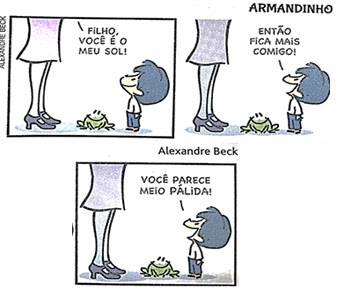
\includegraphics[width=3.51042in,height=3.02083in]{./imgSAEB_7_POR/media/image14.png}

%\fonte{https://tirasarmandinho.tumblr.com/}{\uline{https://tirasarmandinho.tumblr.com/}}.
%Acesso em 20 de Abr de 2023.

\begin{myquote}

Desde que a febre de possuir se apoderou de João Romão totalmente, todos os seus atos, todos, 
fosse o mais simples, visavam um interesse pecuniário. Só tinha uma preocupação: aumentar 
os bens. Das suas hortas recolhia para si e para a companheira os piores legumes, aqueles que,
por maus, ninguém compraria; as suas galinhas produziam muito e ele não comia um ovo, do que, 
no entanto, gostava imenso; vendia-os todos e contentava-se com os restos da comida dos 
trabalhadores. Aquilo já não era ambição, era uma moléstia nervosa, uma loucura, um desespero
de acumular; de reduzir tudo a moeda.

\end{myquote}

\fonte{Aluísio Azevedo. O cortiço.}

No trecho acima, o efeito obtido por meio da personificação da ``febre de possuir'' é descrever

\begin{escolha}
  
  \item a simplicidade do trabalhador João Romão. 
  
  \item a miséria de João Romão e sua companheira.
  
  \item a resignação humilde de João Romão. 
  
  \item a ambição João Romão de acumular bens. 

\end{escolha}


\chapter{Tecendo com as palavras: recursos de coesão e progressão textual}
\markboth{Módulo 10}{}

\section{Habilidades do SAEB}

\begin{itemize}

  \item Analisar os mecanismos que contribuem para a progressão textual.

  \item Analisar os processos de referenciação lexical e pronominal.

\end{itemize}


\subsection{Habilidades da BNCC}

\begin{itemize}

  \item EF07LP12, EF07LP13.

\end{itemize}

\conteudo{A coesão textual é um importante recurso da comunicação escrita.
Para que um texto seja bem escrito e bem compreendido, é necessário que
todas as partes e ideias sejam ordenadas de forma organizada, a fim de
produzir um sentido de conjunto. Para integrar ideias e argumentos que 
compõem um texto, alguns recursos são importantes: conjunções e advérbios, 
por exemplo, servem para estabelecer relações entre ideias, parágrafos, 
orações e frases. Em alguns casos, a fluência da leitura pode
exigir o uso de sinônimos, que vão contribuindo com os sentidos do texto e 
com a coesão ao posicionamento do autor. Pronomes também servem para evitar
a repetição de palavras, evitando a monotonia e trazendo maior objetividade ao texto.

Portanto, a coesão textual é essencial para a produção de um texto claro
e de fácil entendimento. Utilizando os recursos adequados, utilizando palavras 
sinônimas e organizando ideias de maneira linear, é possível criar textos coesos
e bem estruturados, capazes de transmitir as informações de forma eficaz de acordo 
com o contexto, o público, a função comunicativa e o gênero textual que se pretende
produzir.}

% \coment{Professor(a), converse com os estudantes sobre a coesão textual que
% ocorre de maneira imediata na linguagem oral e coloquial. Chame a
% atenção para o uso de expressões repetidas tais como ``daí'', ``então'' e ``né'' 
% na linguagem coloquial e questione o abuso destes termos e o prejuízo
% para a qualidade da comunicação, especialmente a escrita.

% Chame a atenção para os diversos tipos, funções e classes gramaticais de
% palavras que podem ser usadas a fim de contribuir para estabelecer um
% discurso coeso e bem elaborado.}

\section{Atividades}

Leia o texto a seguir para responder às questões de 1 a 3.

\begin{myquote}

A Praça da Sé é o centro geográfico da capital paulista. No local está o Marco Zero 
e é partir dele que são medidas as distâncias das rodovias e fronteiras estaduais, 
assim como a numeração das vias públicas da cidade. Junto à praça está situada a 
Catedral Metropolitana da Sé. Em estilo gótico modificado, sua construção iniciou-se em 1913.
É a maior igreja de São Paulo, com capacidade para oito mil pessoas em seus 110m de comprimento, 
46m de largura, além de torres com 92m e cúpula com 30m de altura. Em sua cripta encontram-se
obras do escultor Francisco Leopoldo.

\end{myquote}

\fonte{Governo do Estado de São Paulo. Praça da Sé. 
https://www.saopaulo.sp.gov.br/conhecasp/pontos-turisticos/praca-da-se/.
Acesso em: 22 mai. 2023.}

\num{1} Na frase ``No \textbf{local} está o Marco Zero e é partir \textbf{dele} que são medidas
as distâncias das rodovias'', a quem se referem os termos destacados?

\reduline{Os termos sublinhados se referem, respectivamente, à Praça da Sé e ao Marco Zero.\hfill}

\num{2} O nome da cidade a que o autor se refere no trecho ``assim como a numeração das vias 
públicas da \textbf{cidade}'' só aparece depois dessa passagem. Explique que cidade é essa e
como foi possível identificá-la no contexto.

\reduline{A cidade a que se refere o autor é a cidade de São Paulo, cujo nome só 
aparce depois do trecho destacado. Ele já havia se referido a essa cidade com a expressão ``capital
paulista''. Além disso,  o contexto em que o texto se insere (o site do governo estadual) também
permite inferir que o autor se refere a São Paulo.\hfill}

\num{3} Quais foram as expressões usadas pelo autor para referir-se à Catedral da Sé?

\reduline{Para referir-se à Catedral da Sé, o autor usou o substantivo ``igreja'' e os pronomes 
possessivos em ``sua construção'', ``seus 110m de comprimento'' e ``sua cripta''.\hfill}

Leia o texto a seguir para responder às questões 4 e 5.

\begin{myquote}

Profissionais da área da educação, da saúde e da assistência social têm
definido ações de cuidado para as comunidades escolares que vivem
situações de violência. Nada fácil, pois a precarização desses setores
tem gerado acúmulo de trabalho e esgotamento.

\end{myquote}

\fonte{Adriana Marcondes Machado. Jornal da USP. Violência às escolas: reflexões. 
Disponível em: https://jornal.usp.br/artigos/violencia-as-escolas-reflexoes/.
Acesso em: 22 mai. 2023.}

\num{4} A expressão ``desses setores'' se refere a que outro termos?

\reduline{A expressão ``desses setores'' se refere às áreas da educação, da saúde e 
da assistência social.\hfill}

\num{5} A expressão ``nada fácil'' se refere a que afirmação?

\reduline{A expressão ``nada fácil'' se refere às ``ações de cuidado para as comunidades escolares que vivem
situações de violência''.\hfill}

Leia o texto abaixo para responder às questões de 6 a 8.

\begin{myquote}

A professora decidiu dividir os alunos do sétimo ano em dois grupos. De um
lado, aqueles que já haviam realizado a prova; de outro, os estudantes que
haviam faltado e que ainda precisavam realizar o exame. Estes deveriam
ser encaminhados para a sala ao lado. O local estava pronto para receber
os estudantes.

\end{myquote}

\num{6} Sublinhe no texto os termos utilizados como recursos de coesão para
evitar repetição dos termos. 

\begin{myquote}
A professora decidiu dividir os alunos do sétimo ano em dois grupos. De um
lado, \textbf{aqueles} que já haviam realizado a prova; de outro, \textbf{os
jovens} que haviam faltado e que ainda precisavam realizar \textbf{o
exame}. \textbf{Estes} deveriam ser encaminhados para a sala ao lado.
\textbf{O local} estava pronto para receber \textbf{os estudantes.}
\end{myquote}


\num{7} O termo \textbf{os jovens} se refere a um termo anterior, restringindo-o. 
Explique essa afirmação.

\reduline{O termo ``os jovens'' se refere ao antecedente ``os alunos'', mas não a todos eles:
apenas aos que haviam faltado.\hfill}

\num{8} O pronome \textbf{estes} se refere a qual grupo de estudantes?

\reduline{O pronome \textbf{estes} se refere aos estudantes que não haviam realizado a prova.\hfill}

\num{9}Complete as lacunas com as palavras do quadro.

\begin{table}[h!]
\begin{tabular}{cc}
obra & garota \\
cujo & ela
\end{tabular}
\end{table}

O livro \_\_\_\_\_\_\_\_ autor Maria conhecia, foi premiado em diversos
concursos literários. A \_\_\_\_\_ tratava das questões que interessavam
a \_\_\_\_\_. A \_\_\_\_\_\_\_\_\_ era uma leitora incansável.

% \coment{O livro \textbf{cujo} autor Maria conhecia, foi premiado em diversos
% concursos literários. A \textbf{obra} tratava das questões que
% interessavam a \textbf{ela}. A \textbf{garota} era uma leitora incansável.}

\num{10} Nas frases abaixo substitua o ponto final por uma conjunção

\begin{escolha}

  \item O clima da cidade é muito árido. Quando vem o período das chuvas a
  vegetação revigora.

\item\reduline{O clima da cidade é muito árido, mas, quando vem o período das chuvas, 
a vegetação revigora.\hfill}
  
  \item O engarrafamento no centro da cidade se prolongou. Houve inundações em
  vários pontos.

\item\reduline{O engarrafamento no centro da cidade se prolongou, pois houve
inundações em vários pontos.\hfill}
  
  \item Adoraria viajar nas minhas férias. Não tenho dinheiro para isso.

\item\reduline{Adoraria viajar nas minhas férias, mas não tenho dinheiro para isso.\hfill}

\end{escolha}

\section{Treino}

\num{1} Leia o texto abaixo para responder à pergunta.

\begin{myquote}

Considerados ``padrão ouro'' nos estudos de saúde, os ensaios clínicos
randomizados controlados, que consistem em testes com voluntários, são a
príncípio aqueles que melhor poderiam mostrar a causalidade entre a
vitamina D e algum efeito na saúde. Mas estudos desse tipo têm
encontrado obstáculos.''

\end{myquote}

\fonte{Mariana Alvim. BBC News Brasil. Vitamina D: o que se sabe e o que 
falta saber sobre suplementos, benefícios e riscos. 
Disponível em: https://www.bbc.com/portuguese/articles/c4nzzzz407xo.
Acesso em: 22 mai. 2023.}

A expressão ``aqueles'' se refere ao antecedente:

\begin{escolha}

  \item ``padrão ouro''.
  
  \item ``estudos de saúde''.
  
  \item ``ensaios clínicos randomizados controlados''.
  
  \item ``estudos desse tipo''. 

\end{escolha}


\num{2} Leia o texto abaixo para responder à pergunta.

\begin{myquote}

A lei alterou as diretrizes e bases da educação nacional para a
inclusão obrigatória do ensino da história e cultura afro-brasileira na
rede pública e particular de ensino fundamental e médio.

\textbf{Conforme o texto}, o conteúdo deve abordar o estudo da história
da África e dos africanos, a luta dos negros no Brasil, a cultura negra
e a participação do negro na formação da sociedade brasileira, nas áreas
social, econômica e política.

\end{myquote}

\fonte{R7 Educação. Mais de 70\% das cidades não cumprem o que manda a lei do
ensino afro-brasileiro nas escolas. 
Disponível em: https://noticias.r7.com/educacao/mais-de-70-das-cidades-nao-cumprem-o-que-manda-a-lei-do-ensino-afro-brasileiro-nas-escolas-20042023.
Acesso em: 22 mai. 2023.}

O trecho em destaque se refere ao antecedente:

\begin{escolha}
  
  \item ``a lei''.
  
  \item ``ensino da história e cultura afro-brasileira''.
  
  \item ``estudo da história da África e dos africanos''.
  
  \item ``a participação do negro na formação da sociedade brasileira''.

\end{escolha}

\num{3} Leia o texto abaixo para responder à pergunta.

\begin{myquote}

Era uma vez um lobo vegano que não engolia a vovozinha, três
porquinhos que se dedicavam à especulação imobiliária e uma estilista
chamada Gretel que trabalhava de garçonete em Berlim. Não deveria nos
surpreender que os contos tradicionais se adaptem aos tempos. Eles foram
submetidos a alterações no processo de transmissão, oral ou escrita, ao
longo dos séculos para adaptá-los aos gostos de cada momento.

\end{myquote}

\fonte{Marta Rebós. El País Brasil. O lobo devorou, sim, a Chapeuzinho.}

% \fonte{Marta Rebós. El País Brasil. O lobo devorou, sim, a Chapeuzinho. 
% https://brasil.elpais.com/brasil/2018/09/18/eps/1537265048_460929.html
% Acesso em: 22 mai. 2023.}

No útlimo período do texto, os termos destacados em ``\textbf{Eles} foram
submetidos a alterações'' e ``para adaptá-\textbf{los} aos gostos'' se referem:

\begin{escolha}

  \item aos antecedentes ``lobo vegano'' e ``três porquinhos''.

  \item ambos ao antecedente ``três porquinhos''. 

  \item ambos ao antecedente ``contos tradicionais''.

  \item aos antecedentes ``contos tradicionais'' e ``séculos''.

\end{escolha}


\chapter{Variedades linguísticas}
\markboth{Módulo 11}{}

\section{Habilidades do SAEB}

\begin{itemize}

  \item Analisar as variedades linguísticas em textos.

  \item Avaliar a adequação das variedades linguísticas em contextos de uso.

\end{itemize}

\subsection{Habilidades da BNCC}

\begin{itemize}

  \item EF69LP55, EF69LP56.

\end{itemize}


% conteudo não funciona aqui
A língua é um fenômeno social complexo que se manifesta de diversas
maneiras, de acordo com o contexto. As várias
formas de uso da língua são chamadas de \textbf{variedades linguísticas}, e estão
presentes nas diferenças de pronúncia, vocabulário e situação
comunicativa.

Existem muitas variações da língua falada, pois a linguagem é
influenciada por fatores como a região onde se encontram determinadas
expressões, o nível de escolaridade, a idade, a classe social e a etnia
dos falantes. As variações linguísticas podem ser referentes
ao uso coloquial ou formal, ao uso profissional, ou depender de aspectos
geográficos e históricos. Por esses motivos, as variações
se diferenciam da chamada norma-padrão.

Contudo, mesmo que a diversidade seja uma característica
inerente à linguagem, as variações linguísticas podem sofrer preconceitos
e discriminação. Por outro lado, conhecê-las permite a criação de um
discurso mais acessível e atento ao público a que se dirige. No entanto,
considerar determinadas formas de uso da língua inferiores ou
equivocadas pode ser considerado preconceito linguístico.

O preconceito linguístico pode ter diversas consequências negativas,
como a exclusão social de falantes de determinadas variedades
linguísticas, pois não são levados em conta diversos fatores como a
dificuldade de acesso e de oportunidades educacionais e profissionais.

Portanto, é importante valorizar e respeitar a diversidade linguística
como um patrimônio cultural e expressivo que considera todos os falantes
da língua, combatendo os preconceitos e promovendo a inclusão social.

\section{Atividades}

\num{1} Quais são os fatores que devem ser considerados para compreender as
variações linguísticas existentes entre os falantes de uma mesma

\reduline{Para compreender as variações linguísticas, é preciso levar em 
consideração fatores sociais, nível de escolaridade, poder aquisitivo, 
peculiaridades culturais, étnicas e regionais.\hfill} 

\num{2} Por que a desvalorização de determinados usos da linguagem pode ser
considerada preconceito?

\reduline{A desconsideração das questões que promovem as variações linguísticas
induz ao preconceito, pois não se pode desconsiderar o contexto do
emissor e nem a situação comunicativa. Em muitos casos, a norma-padrão
não se apresenta como a forma mais eficaz de elaborar um texto ou
discurso. Além disso, a norma-padrão pode servir à manutenção da desigualdade
social, especialmente em países como o Brasil.\hfill} 

Leia um trecho do romance \textit{Dom Casmurro}, de Machado de Assis:

Capitu deixou-se ir, rindo; depois a conversa entrou a cochilar e
dormir. Tínhamos chegado à janela; um preto, que, desde algum
tempo, vinha apregoando cocadas, parou em frente e perguntou:

--- Sinhazinha, qué cocada hoje?

--- Não, respondeu Capitu.

--- Cocadinha tá boa.

--- Vá-se embora, replicou ela sem rispidez.

--- Dê cá! disse eu descendo o braço para receber duas.

Comprei-as, mas tive de as comer sozinho; Capitu recusou. Vi
que, em meio da crise, eu conservava um canto para as cocadas, o
que tanto pode ser perfeição como imperfeição, mas o momento
não é para definições tais; fiquemos em que a minha amiga,
apesar de equilibrada e lúcida, não quis saber de doce, e gostava
muito de doce. Ao contrário, o pregão que o preto foi cantando, o
pregão das velhas tardes, tão sabido do bairro e da nossa infância:



\begin{verse}
Chora, menina, chora, \\
Chora, porque não tem \\
Vintém
\end{verse}


\fonte{Machado de Assis. Dom Casmurro. 
Disponível em: https://www.ic.unicamp.br/~stolfi/misc/2012-02-13-domine-casmurrus.pdf.
Acesso em: 22 mai. 2023.}

\num{3} No diálogo entre o vendedor de cocadas, de um lado, e Capitu e Bentinho, 
o narrador do romance, de outro, é possível perceber variações linguísticas. 
Explique essas variações, considerando que, no período em que se passa o romance, o 
vendedor é uma pessoa escravizada no Brasil de meados do século XIX, ao contrário do 
narrador e Capitu, que são brancos com acesso à educação formal. 

\reduline{Fica evidente no diálogo entre o vendedor de cocadas e Capitu e Bentinho que
o abismo social entre essas personagens se manifesta nas variações linguísticas. Enquanto
as falas de Capitu e Bentinho tendem à norma-padrão (por exemplo, no uso do pronome em 
``vá-se embora''), as do vendedor se aproximam da informalidade oral, como em 
``qué cocada hoje?'' e ``Cocadinha tá boa''.\hfill}

\num{4} Nos parágrafos do narrador, qual é a variedade linguística predominante? 
Copie um exemplo de uso de pronomes que confirma essa explicação. 

\reduline{O uso dos pronomes pessoais oblíquos átonos em ``Comprei-as, mas tive de 
as comer sozinho'' corresponde à norma-padrão. Em variedade linguística menos rigorosa,
e mais natural para muitos falantes de língua portuguesa do Brasil, seria usado o pronome
``elas''.\hfill} 

\num{5} O que são os \textbf{pregões} citados pelo narrador? Ainda existem pregões no
seu cotidiano? Se sim, explique; se não, levante hipóteses sobre o desaparecimento dessa 
prática.

\reduline{Pregões são divulgações em voz alta de produtos à venda, por vendedores ambulantes. 
Feirantes de rua ainda costumam usar pregões, bem como vendedores ambulantes nas praias de 
todo o Brasil. Contudo, o ambiente do comércio em shopping centers, mais formal, não contempla
essa prática.\hfill} 

%Analise a tirinha e responda:

%
\includegraphics[width=5.90551in,height=1.70833in]{./imgSAEB_7_POR/media/image15.png}

%\num{6}
%  A tirinha apresenta um tipo de variação linguística? Justifique sua resposta
%\end{enumerate}

%Sim. A tirinha apresenta uma variação linguística pois apresenta vários
%nomes de um mesmo vegetal, cada forma é utilizada em uma região
%diferente do país

%\num{7}
%  Alguma das formas mandioca, aipim ou macaxeira pode ser considerada
%  mais correta do que as outras? Por que?
%\end{enumerate}

%Não, pois cada região possui suas formas de falar, suas gírias e
%expressões e muitas vezes, podem haver vários sinônimos em uma mesma
%língua usado em regiões e culturas diferentes.

\num{6} Na tabela a seguir, assinale (V) para as afirmações verdadeiras e (F) para as falsas no que
se refere às variedades linguísticas. 

\begin{table}[h!]
\begin{tabular}{|c|c|}
\hline
\textbf{\begin{tabular}[c]{@{}c@{}}Verdadeiro (V)\\ ou Falso (F)?\end{tabular}} & \textbf{Afirmação} \\ \hline
\rosa{F} & toda situação comunicativa exige o uso da norma-padrão \\ \hline
\rosa{V} & \begin{tabular}[c]{@{}c@{}}o uso da norma-padrão é mais adequado para a redação de\\ documentos oficiais, textos de lei e petições\end{tabular} \\ \hline
\rosa{F} & textos literários devem sempre fazer uso da norma-padrão \\ \hline
\rosa{V} & em algumas situações, é mais adequado não utilizar a norma-padrão \\ \hline
\rosa{V} & \begin{tabular}[c]{@{}c@{}}a escolha pelo uso da norma-padrão ou de variações que se distanciam dela\\  deve orientar-se pelo contexto da comunicação\end{tabular} \\ \hline
\end{tabular}
\end{table}

% Gabarito: \coment{F, V, F, V, V}

\num{7} Na tabela abaixo, assinale com um X os gêneros textuais em que o uso da norma-padrão 
tende a ser mais adequado.

\begin{table}[h!]
\begin{tabular}{l|l|}
\cline{2-2}
 & \textbf{Gêneros textuais} \\ \hline
\multicolumn{1}{|l|}{} & cartas pessoais \\ \hline
\multicolumn{1}{|l|}{\rosa{x}} & cartas abertas à sociedade \\ \hline
\multicolumn{1}{|l|}{\rosa{x}} & petições \\ \hline
\multicolumn{1}{|l|}{\rosa{x}} & textos de divulgação científica \\ \hline
\multicolumn{1}{|l|}{\rosa{x}} & leis e estatutos \\ \hline
\multicolumn{1}{|l|}{} & poemas \\ \hline
\end{tabular}
\end{table}

\num{8} Na tabela abaixo, assinale com um X as situações comunicativas em que tende a ser mais adequado
o uso da linguagem coloquial.

\begin{table}[h!]
\begin{tabular}{l|l|}
\cline{2-2}
 & \textbf{Situações comunicativas} \\ \hline
\multicolumn{1}{|l|}{\rosa{x}} & conversa com amigos \\ \hline
\multicolumn{1}{|l|}{} & matérias de jornal \\ \hline
\multicolumn{1}{|l|}{} & apresentação de trabalho escolar \\ \hline
\multicolumn{1}{|l|}{\rosa{x}} & mensagens de redes sociais \\ \hline
\end{tabular}
\end{table}

\section{Treino}

\num{1} Leia os versos do coco abaixo para responder à questão.

\begin{myquote}
\begin{verse}

Eu vi uma lagartixa \\
Ai, tava numa jinela, \\
Ai, dizeno que era honrada, \\
Que era moça donzela, \\
Vi quat' calango verde, \\
Tudo era fio dela. 

\end{verse}
\end{myquote}

\fonte{Mário de Andrade. Os cocos. Belo Horizonte: Itatiaia, 2002. p. 157.} 

O coco é uma dança popular de roda, que se executa ao som de canto, batida de palmas e 
toque de percussão. Nos versos acima, registrados pelo escritor e pesquisador Mário de 
Andrade, observa-se a transcrição da fala coloquial em:

\begin{escolha}
  
  \item ``eu vi''.
  
  \item ``era honrada''.
  
  \item ``donzela''.
  
  \item ``fio dela''

\end{escolha}


\num{2} Leia o texto abaixo para responder à questão.

\begin{myquote}
Nota-se também que as diferentes regiões brasileiras não apresentam um
cenário socioeconômico igual, o que afeta a frequência do câncer e de
outras doenças. ``Pensar em regionalização é essencial. Nas regiões Norte
e Nordeste, por exemplo, esse tipo de câncer não é tão frequente como em
outros espaços do País. Quando você pensa em um projeto de prevenção, é
necessário pensar em regionalização'', discorre Hoff.''
\end{myquote}

\fonte{Jornal da USP. Câncer de intestino já é mais comum em grupos de pessoas mais jovens.
Disponível em: https://jornal.usp.br/radio-usp/cancer-de-intestino-ja-e-mais-comum-em-grupos-de-pessoas-mais-jovens/.
Acesso em: 22 mai. 2023.}

No exemplo acima, o autor usou da norma-padrão para adequar-se à linguagem apropriada ao texto

\begin{escolha}
  
  \item literário.
  
  \item humorístico.
  
  \item jornalístico.
  
  \item jurídico.

\end{escolha}

\num{3} Leia o trecho do romance \textit{A Família Medeiros}, de Júlia Lopes de Almeida, para 
responder à questão. 

\begin{myquote}

Passada a curva do jequitibá grande, topou com um negro
que vencia o morro a largas passadas e que o saudou com um
soturno:
--- Sum Cristo!
--- Sabe-me dizer se há algum atalho novo para a Fazenda de
Santa Genoveva?
--- Prá o sito do coroné Medêro? Não há não, sinhô. Eu
também tô indo prá lá.
E atentando em Otávio:
--- A modo qui tô conhecendo mecê \ldots{}
--- Está, sim. E você, como se chama?
--- Me chamo Antonho; fio de Luzia pernambucana, sim sinhô.
--- Foi a algum recado à cidade?
--- Fui na vila buscá rémedio pró fio do feitô, qui foi moldido
de cobra, sim sinhô \ldots{}
--- Ah, então apresse-se --- disse Otávio, para dizer alguma
coisa, e tocou o animal para diante.
\end{myquote}


\fonte{Júlia Lopes de Almeida. A Família Medeiros. São Paulo: Editora Hedra. no prelo.}

No diálogo acima, observa-se a transcrição da fala coloquial em:

\begin{escolha}
  
  \item ``vencia o morro a largas passadas''.
  
  \item ``Sabe-me dizer se há algum atalho novo''. 
  
  \item ``A modo qui tô conhecendo mecê''.
  
  \item ``então apresse-se''. 

\end{escolha}
